\chapter{Tackling Spatial Continuity: Task-Specific Region Partition}
\label{ch:partition}

In this chapter, I focus on the second challenge in region networks modeling, i.e. how to construct discrete nodes from continuous spatial space. We formulate our problem as an NP-hard combinatorial optimization problem. 

% !TEX root =  main.tex
\section{Introduction}

% More data are available
Recent years have seen more and more cities join the open data initiative. For example, as of December 2016, more than 1600 data sets are available on  NYC open data catalog \cite{nyc-open-data}. These public urban data collectively reflect urban dynamics and provide a unique opportunity to fully engage the data-informed city. 

% model

Given the growing amount of urban data, a number of data-driven models have been developed to provide insights for urban problems. A frequent approach is to treat each region as a data sample, take the region properties as features, and build a model to learn the correlation between region features and a target variable. One common application lies in the domain of crime prediction. Criminologists are interested in knowing the correlation between demographics and crime~\cite{wang2016crime,wang2017non}. Each region $i$ is taken as a data sample, with $X_i$ as its demographic feature and $Y_i$ as its crime count. A model (e.g., linear regression or negative binomial model) is built to estimate crime count vector $Y$ using the feature matrix $X$. If some features (e.g., disadvantage index) show a significant correlation with crime count, researchers could relate this empirical result with criminology theory~\cite{graif2014urban} and policy makers could further propose corresponding policies to address crime issues.

Existing studies often use pre-defined administrative boundaries (e.g., street block, census tract, community area, or neighborhood) to define a region~\cite{yuan2012discovering,wang2016crime}. An example of the 77 administrative community areas of Chicago is shown in Figure~\ref{fig:intro}. However, such administrative boundaries might be too rigid and do not reflect the true spatial structure with regards to the targeted urban issues. For example, the definition of regions for crime study might be different from the regions used to understand real estate market. One can alternatively propose to study the problem at the point level or small grid cell level (e.g., 10 meters by 10 meters grids). However, this could lead to data sparsity issues and jeopardize the integrity of the statistical model. Consequently, any inference made from the model would be at risk of bias. These concerns have both theoretical and policy implications. We use the following example to further illustrate the issue of using pre-defined community areas to study crime.

\begin{figure}[t]
\centering
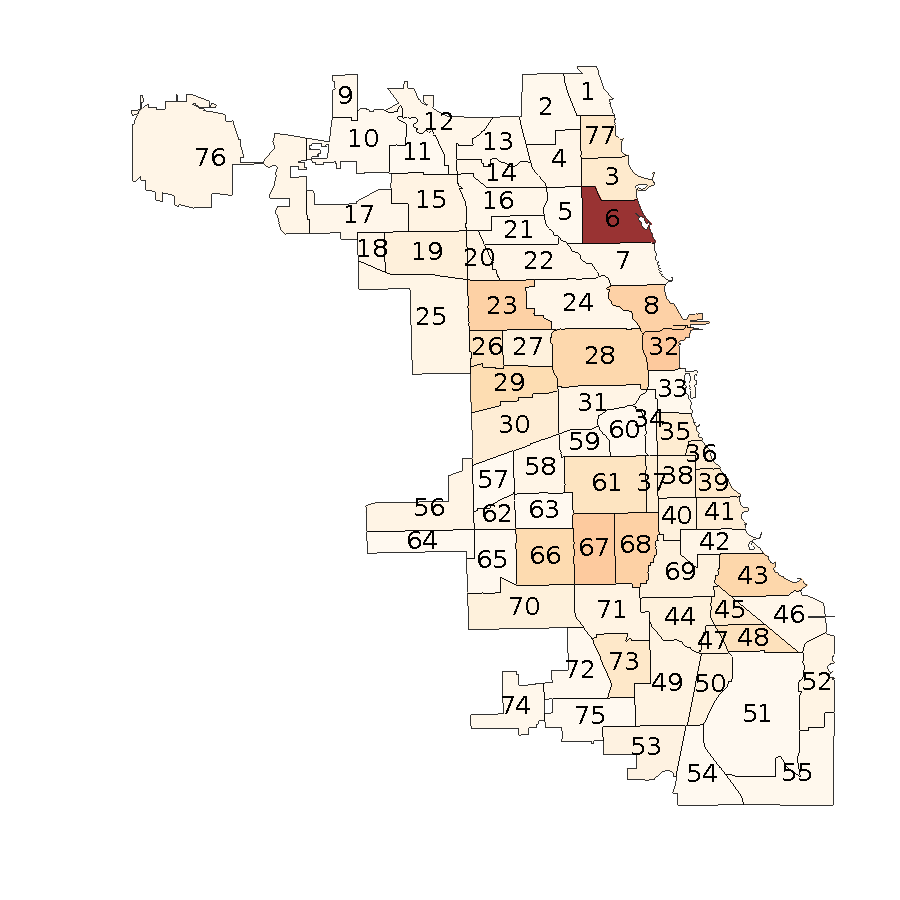
\includegraphics[width=0.4\linewidth]{fig/error_heatmap.pdf}
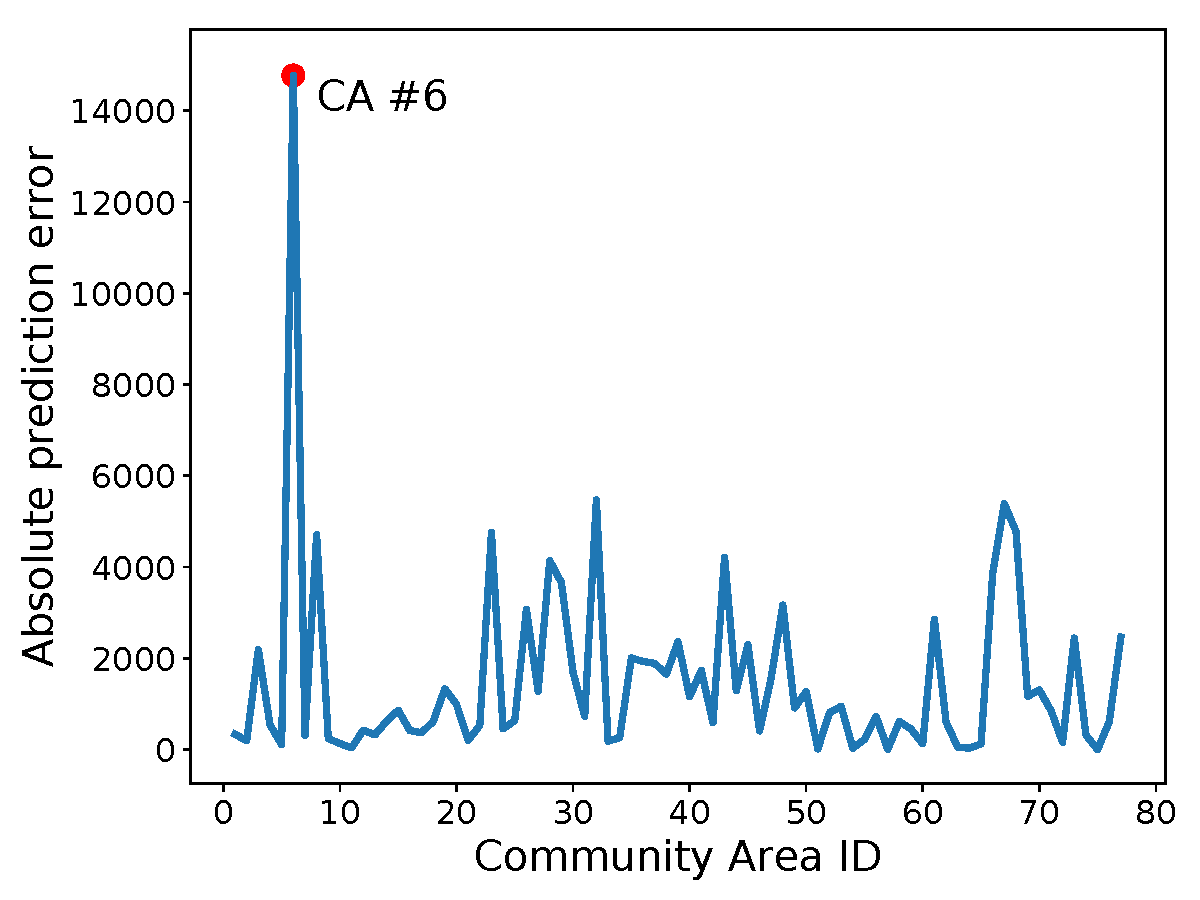
\includegraphics[width=0.5\linewidth]{fig/ca-abs-errors.pdf}
\caption{Crime prediction error at community level in Chicago. The community area \#6 is an outlier with a large error.}
\label{fig:intro}
\end{figure}

\begin{figure}
\centering
\subfigure[Census tracts of community \#6.]{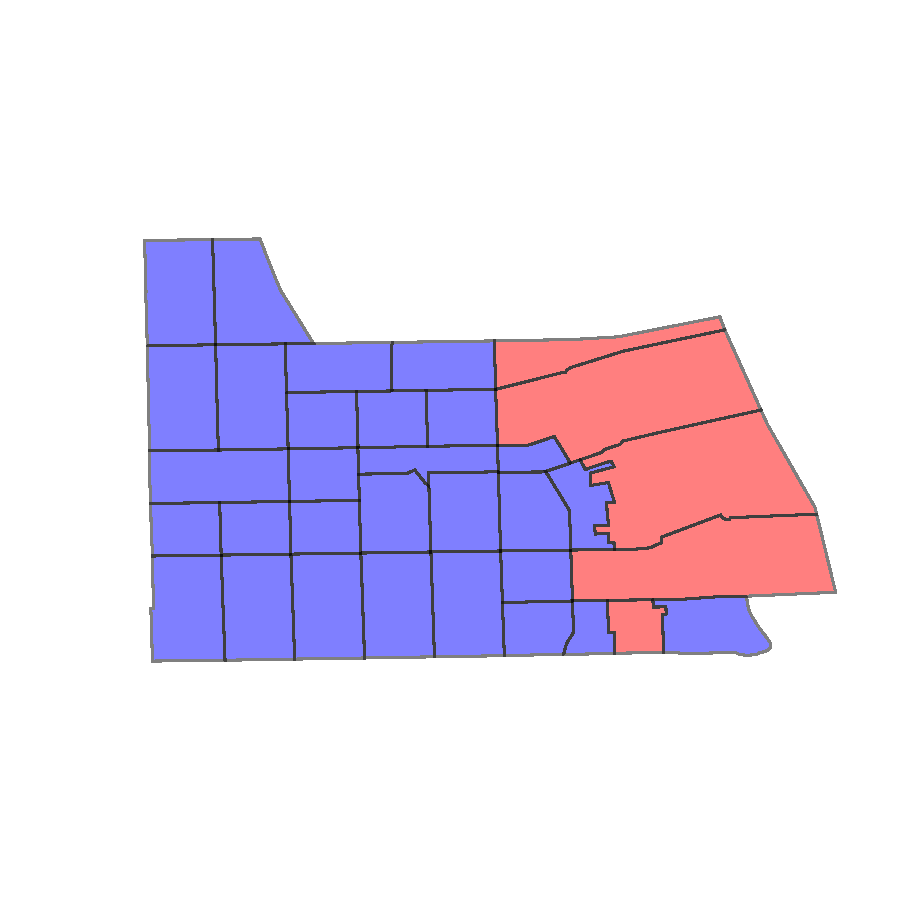
\includegraphics[width=0.5\linewidth]{fig/tracts_within_CA.pdf}}
\subfigure[Tract similarity.]{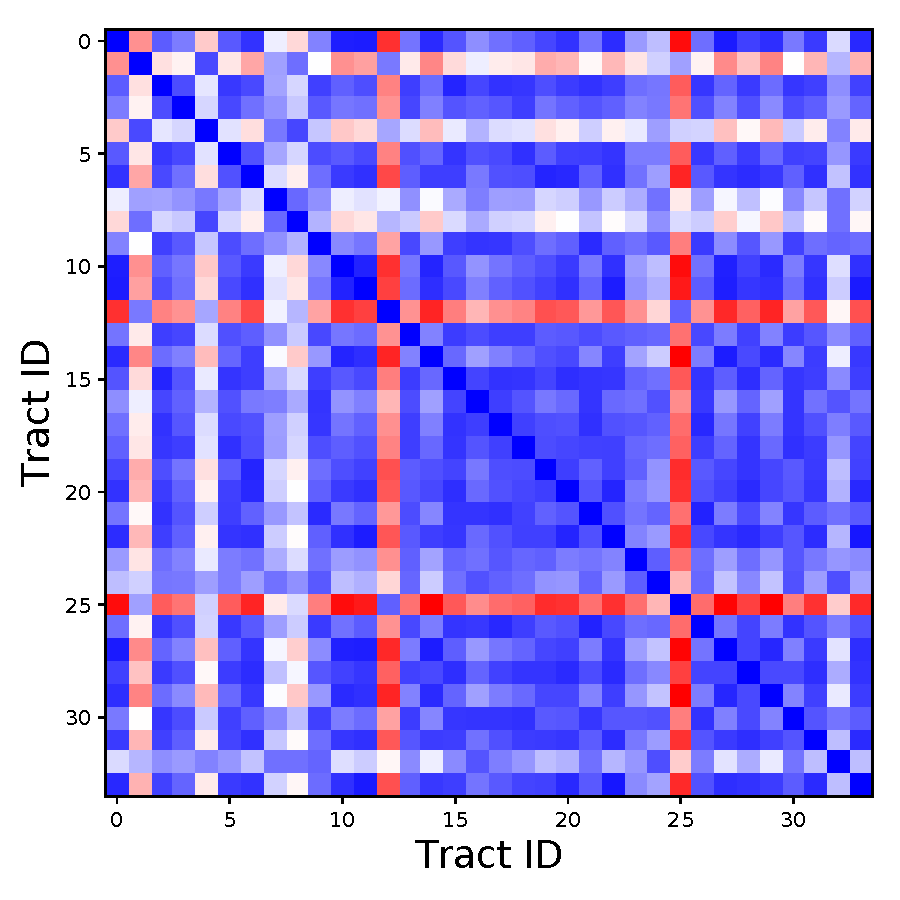
\includegraphics[width=0.45\linewidth]{fig/tract_sim_matrix.pdf}}
\caption{Explaining the outlying community area \#6 in Figure~\ref{fig:intro}. (a) Visualization of the 34 tracts in community \#6. (b) The pair-wise similarity of 34 tracts in terms of demographic features. It is clear that five tracts (in red color) on the east side are different from the other blue tracts.}
\label{fig:intro-explain}
\end{figure}

\begin{example}
Following previous work~\cite{wang2016crime}, we construct a negative binomial model to predict crime count using demographic features by treating each community area as a data sample. Figure~\ref{fig:intro} plots the crime prediction error for each community area of Chicago. Community area \#6 (i.e., Lake View area) shows an abnormally high error. In order to explain this outlier, we further investigate the internal structure of this area. Community \#6 consists of 34 census tracts as shown in Figure~\ref{fig:intro-explain}(a).  In Figure~\ref{fig:intro-explain}(b), we visualize  pair-wise Euclidean distance between tracts based on demographic features. There are five tracts that are different from the other tracts in the demographic feature space, and they are all located on the east side of community \#6. These five tracts, when mixed with other tracts in this community, lead to inferior performance of crime count prediction in that area. 
\end{example}

% problem definition
The observation above motivates us to learn a better region definition for crime study. In this chapter, we propose a new problem of \emph{task-specific region partitioning}. Given spatial variables and a selected model  (e.g., linear regression), we aim to partition the city into regions such that the model trained by taking regions as data samples achieves the optimal results.

% literature
%two lines of literature: (1) clustering, no target; (2) partition tracts into regions, and build a model for each region.
To the best of our knowledge, task-specific region partitioning is a new problem that has not been studied before. While there exist many methods for spatial clustering~\cite{miller2009geographic}, most of them group the locations based on the similarity of their spatial properties and do not have a target variable to predict. Another similar problem is to partition the locations into $k$ regions and fit a model for each region. Such a problem definition has a different purpose with the goal of showing that the correlations between features and target vary over the space (e.g., in some area, disadvantage index  correlates with crime; while in some other areas, it does not). In our problem definition, we aim to fit one model for the whole city hoping to get a generalized interpretation (e.g., disadvantage index significantly correlates with crime count in Chicago). Such a problem definition is a frequently adopted form in the criminology literature~\cite{graif2014urban}.

% challenge & proposed solution
Task-specific city region partitioning is a challenging problem. The key challenge lies in that the region properties (both features and target variable) and the model coefficients change simultaneously when we change the region partition. We prove that this is an NP-hard problem. In our proposed solution, we employ the Markov Chain Monte Carlo (MCMC) method. We start from a pre-defined region partition (e.g., community areas), and generate a new partition sample by flipping the membership of a smaller area (e.g., a tract). Two variants of MCMC methods are proposed to solve this problem. First, a naive MCMC method generates the next partition sample by randomly flipping a tract. Second, a heuristic-based MCMC method generates the next sample by flipping one tract randomly selected from the community areas with the highest error. Finally, we employ reinforcement learning to automatically learn how to generate the next sample that is more likely to improve the prediction performance.


% Experiments results
We evaluate our method on two real datasets, i.e. crime count and real estimate price. The learned region partitions are shown to consistently outperform the administrative boundaries and spatial clustering method. For example, our methods, on average, outperform the administrative boundary by $56\%$ in a crime prediction task. We also observe that the heuristic-based MCMC converges faster than the naive MCMC, while the reinforcement learning uses the least iterations to converge.

% Key contributions
To summarize, the key contributions of this chapter are:
\begin{itemize}[leftmargin=*]
\item We propose a novel problem on task-specific region partitioning. This problem is motivated by real-world urban studies, including our own previous work on crime prediction~\cite{wang2016crime}.
\item We prove the problem is NP-hard and we study different MCMC and reinforcement learning sampling techniques to solve the problem. 
\item We validate our method through extensive experiments on two real datasets.
\end{itemize}


% chapter organizations
The rest of this chapter is organized as follows. The formal definition of our problem is given in Section~\ref{ch4-sec:problem}, and our method is described in Section~\ref{ch4-sec:method}. Section~\ref{ch4-sec:experiment} shows the evaluations on two different tasks. Section~\ref{ch4-sec:related-work} summarizes related work.  Finally, we conclude in Section~\ref{ch4-sec:conclusion}.


\section{Region Partition Problem}
\label{ch4-sec:problem}

In this section, we first present the formal definition of our method. Then we prove that this partition problem is NP-hard.


The input of our problem is a set of minimum spatial units. Without loss of generality, we use tract as the unit of study in this paper, and the set of tracts is denoted as $\mathcal{T} = \{ t_1, t_2, \cdots, t_n \}$. Within each tract $t_i$, the following information are available $\langle p_i, y_i, x_i \rangle$, where $p_i$ is a sequence of GPS coordinates representing tract exterior boundary, $y_i$ is the target variable of interest, such as crime count and average house price, and $x_i \in \mathcal{R}^d$ is a $d$-dimension contextual feature vector. Note that each tract is a polygon with one connected component.

We define community area as the proper unit to study the correlation between $y$ and $x$.
\begin{definition}[Community area]
 Each community area consists of several adjacent tracts, denoted as $Z_j = \{t_1^j, t_2^j, \cdots \}$. We derive $\langle P_j, Y_j, X_j \rangle$ for each community area $Z_j$ by aggregating $\{ \langle p_i, y_i, x_i \rangle | t_i \in Z_j \}$, where $P_j$ is the exterior boundary, $Y_j$ is the crime count, and $X_j$ is the contextual features of $Z_j$.
\end{definition}
Note that there are various approaches to aggregate tract-level features $x_i$ into community area features $X_j$. For example we can use element-wise summation, min, or max on categorical count features. We can also calculate entropy to derive a diversity feature as $X_j$.

With the definition of community area, we define the partition of a city.
\begin{definition}[Partition]
\label{def:partition}
A partition over $\mathcal{T}$ is denoted as $\mathcal{Z} = \{ Z_1, Z_2, \cdots, Z_m\}$, satisfying the following four conditions
\begin{enumerate}
\item (subset) $\forall j$, $Z_j \subset \mathcal{T}$;
\item (non-overlapping) $\forall p, q$, $Z_p \cap Z_q = \emptyset$;
\item (completeness) $\bigcup_{j=1}^m Z_j = \mathcal{T}$;
\item (spatial-continuity) $\forall j$, $P_j$ defines a polygon with exact one connected component.
\end{enumerate}
\end{definition}

A task is defined on a given partition of the city, where we aim to learn the correlation between $X$ and $Y$ at the community area level.
\begin{definition}[Task]
Given a partition $\mathcal{Z}$, a task is to learn a linear function $f$, such that $Y_j = f(X_j)$, 
where $X_j$ and $Y_j$ are target variable and contextual features of community area $Z_j$.
\end{definition}


Our ultimate goal is to have a more accurate prediction. The task-specific region partition problem is defined as follows.
\begin{definition}[Task-specific region partition]
\label{def:opt-problem}
Given a set of tracts $\mathcal{T}$ and a task $f$, find a partition $\mathcal{Z}$ with $m$ components, such that the task error is minimized. Formally, we have
\begin{equation}
\label{eq:objective}
\arg\min_{\mathcal{Z}, f} \sum_{j=1}^m \Big(||Y_j - f(X_j)||_2 + G(Z_j)\Big),
\end{equation}
where $G(\mathcal{Z}) = \sum_{j=1}^m G(Z_j)$ is a constraint function on partition.
\end{definition}

The constraint function $G$ ensures the partition $\mathcal{Z}$ has desirable property, such as small variance in community populations or balanced size in terms of community area. \\


\noindent\textbf{NP-Hardness}. The problem in Definition~\ref{def:opt-problem} is a combinatorial optimization problem, where the set of instances is $\mathcal{T}$, the feasible solution is $\mathcal{Z}$, and the quality measure of solution is $\mathcal{F}(\mathcal{Z}, f) = \sum_{j=1}^m \mathcal{F}(Z_i, f)$. The decision version of the problem is to find a partition $\mathcal{Z}$, such that $\mathcal{F}(\mathcal{Z}, f) \leq \epsilon$, where $\epsilon$ is a constant. In this section, we prove such decision problem is NP-complete, and therefore the optimization problem in Definition~\ref{def:opt-problem} is NP-hard.

In the NP-completeness proof, we approximate the decision problem above with an easier problem. The reason is that both $X_i$, $Y_i$, and $f$ are dynamically changing according to $\mathcal{Z}$, which complicates the original problem. First, we replace the jointly learned optimal $f$ with a fixed $f_0$. Since $f$ is optimal to minimize Equation~\ref{eq:objective} while $f_0$ is not, we have $\mathcal{F}(\mathcal{Z}, f) < \mathcal{F}(\mathcal{Z}, f_0)$. Second, we use $\sup \{\mathcal{F}(Z_j, f_0) \}$, where $\sup$ calculates supremum of a set, to approximate $\mathcal{F}(\mathcal{Z}, f_0)$. Since there are finite number of tracts within each community $Z_j$, and the task function $f_0$ can be solved in polynomial time, therefore the upper bound of $\mathcal{F}(Z_j, f_0)$ exists and is finite. Combine two approximations above, we have $\mathcal{F}(\mathcal{Z}, f) < m \cdot \sup \{ \mathcal{F}(Z_j, f_0)\}$. The approximated decision problem is to find a partition $\mathcal{Z}$, such that $m \cdot \sup \{\mathcal{F}(Z_j, f_0) \} \leq \epsilon_0$.

Now we prove the approximated decision problem is NP-complete. First, such approximated decision problem is NP, because given a partition $\mathcal{Z}_0$, we are able to validate $m \cdot \sup \{ \mathcal{F}(Z_j, f_0)\} \leq \epsilon_0$ in polynomial time. Next, we prove the NP-hardness of this problem by reducing the $(k,v)$-balanced partitioning problem to the approximated decision problem. The $(k,v)$-balanced partition problem~\cite{andreev2006balanced} is a proved NP-complete problem, which partition graph into $k$ disjoint components of size at most $v\frac{n}{k}$, while the capacity of edge cut is less than $\epsilon_0$. We construct the adjacency graph of all tracts $\mathcal{T}$, with weight $\sup \{\mathcal{F}(Z_j, f_0) \}$ on each edge. A solution to $(m,v)$-balanced partition problem on such adjacency graph is a solution to the approximated decision problem. The balanced partition problem achieve $k \cdot \sup \{\mathcal{F}(Z_j, f_0) \} \leq \epsilon_0$, where $k$ is the number of edges to cut the graph. It is clear that $k > m$, and therefore we find a partition satisfying $m \cdot \sup \{ \mathcal{F}(Z_j, f_0)\} \leq \epsilon_0$. 

The original problem in Definition~\ref{def:opt-problem} is NP-hard. Therefore, it is difficult to efficiently search for the optimal partition. In this paper, we use Markov Chain Monte Carlo sampling strategy to search for local optimal solutions.

\section{methods}
\label{sec:method}

In this section, we use the stochastic Markov Chain Monte Carlo (MCMC) method to automatically learn the partition $\mathcal{Z}$. We propose two variations of MCMC sampling method with different sample proposal strategy. And finally, we use reinforcement learning to make the best of historical samples and automatically learn the sample strategy.


\subsection{Markov Chain Monte Carlo}

There are two parameters, $\mathcal{Z}$ and $f$, to learn in Equation~\ref{eq:objective}. However, given a fixed partition $\mathcal{Z}$, the optimal task function $f$ can be easily learned. The challenge lies in searching through the partition space. Toward this goal, we adopt the MCMC method, or more specifically the Metropolis-Hastings algorithm to optimize $\mathcal{Z}$. 

Markov Chain Monte Carlo~\cite{andrieu2003introduction} is a stochastic algorithm for obtaining a sequence of random samples from a distribution for which direct sampling is difficult. A key property of the algorithm is that it constructs a Markov chain that will ultimately converge to $p$ through stochastic sampling \cite{ml:murphy}. In our case, the state space is all possible partitions $\mathcal{Z}$, and the distribution $p(\mathcal{Z})$ defines the probability that $\mathcal{Z}$ is optimal to Problem~\ref{def:opt-problem}. Clearly, it is difficult to calculate $p(\mathcal{Z})$, however the quality measure $\mathcal{F}(\mathcal{Z})$ is proportional to $p(\mathcal{Z})$. Namely, a partition $\mathcal{Z}$ with lower $\mathcal{F}(\mathcal{Z})$ value is more likely to be optimal.


In addition to the quality function $\mathcal{F}$, MCMC employs a proposal function $q(\mathcal{Z}'|\mathcal{Z})$, which defines the transition probability from state $\mathcal{Z}$ to $\mathcal{Z}'$. The Markov chain moves toward $\mathcal{Z}'$ with acceptance probability $\gamma$, defined as
\begin{equation}
\gamma = \min \Big [ 1, \frac{p(\mathcal{Z}')q(\mathcal{Z}| \mathcal{Z}')}{p(\mathcal{Z})q(\mathcal{Z}'|\mathcal{Z})} \Big ].
\label{eq:gamma}
\end{equation}

$p(\mathcal{Z})$ is the Boltzmann distribution, defined by
\begin{equation}
p(\mathcal{Z}) = \frac{e^{-\mathcal{F}(\mathcal{Z})/T}}{P}, 
\label{eq:boltzmann}
\end{equation}
where $P$ is the normalization constant, and $T$ is the temperature parameter. We do not explicitly compute $P$, because they cancel out in Equation~(\ref{eq:gamma}).

\begin{algorithm}
\caption{MCMC method to search $\mathcal{Z}$.}
\label{alg:mcmc}
\begin{algorithmic}[1]
\State $\mathcal{Z} \gets \mathcal{Z}_0$
\While {$\mathcal{F}(\mathcal{Z}) \geq \epsilon$}
  \State Sample $u \gets \mathcal{U}_{[0,1]}$
  \State Sample $\mathcal{Z}' \gets q(\mathcal{Z}'|\mathcal{Z})$
  \State $\gamma = \min \Big [ 1, \frac{p(\mathcal{Z}')q(\mathcal{Z}| \mathcal{Z}')}{p(\mathcal{Z})q(\mathcal{Z}'|\mathcal{Z})} \Big ]$
  \If {$u < \gamma$}
    \State $\mathcal{Z} \gets \mathcal{Z}'$
  \EndIf
\EndWhile
\end{algorithmic}
\end{algorithm}

The MCMC algorithm is shown in Algorithm~\ref{alg:mcmc}. First, we initialize the partition with the existing administrative boundary, denoted as $\mathcal{Z}_0$. Within each step, we draw $u \in [0,1]$ from uniform distribution $\mathcal{U}_{[0,1]}$, and draw the next partition $\mathcal{Z}'$. The acceptance probability $\gamma$ is calculated according to Equation~\ref{eq:gamma}. If $u$ is smaller than the acceptance probability $\gamma$, then we accept the new partition $\mathcal{Z}'$. We repeat the process above, until $\mathcal{F}(\mathcal{Z})$ converges.



\subsection{MCMC with Naive Proposal Distribution}

The proposal function $q$ is very flexible, if not limitless. In practice, the exact form of $q$ generally affects the efficiency of the algorithm, or how quickly it will converge. We begin by establishing a baseline MCMC approach to the region partition problem by outlining the simplest $q$ we can devise. 

We generate a new partition by randomly selecting one tract $t_i \in \mathcal{T}$ that is on the boundary of some community area $Z_j$, and then flip $t_i$ to the adjacent community area. Such a naive proposal function $q$ contains the following steps.
\begin{itemize}
  \item Maintain a set of tracts that are on partition boundary, denoted as $\mathcal{T}_b$.
  \item Uniformly draw $t_i$ from $\mathcal{T}_b$. The current community assignment for $t_i$ is $Z_j$. The probability of selecting $t_i$ is $1/|\mathcal{T}_b|$.
  \item Uniformly draw $Z_p$ from the set of adjacent community areas $Adjacent(t_i)$ of $t_i$. The probability of selecting $Z_p$ is $1/|Adjacent(t_i)$.
  \item Verify the four conditions in Definition~\ref{def:partition} are satisfied. If not, restart.
  \item Assign the $t_i$ to community $Z_p$. Update boundary set $\mathcal{T}_b$.
\end{itemize}

The naive proposal function $q$ is symmetric, because $q(\mathcal{Z}'|\mathcal{Z})=  q(\mathcal{Z}|\mathcal{Z}') = \frac{1}{|\mathcal{T}_b| \cdot |Adjacent(t_i|}$. Therefore, the acceptance probability $\gamma = \min[ 1, \frac{p(\mathcal{Z}')}{p(\mathcal{Z})}]$. 


\subsection{Guided MCMC with Softmax Proposal Distribution}

The naive proposal MCMC method is simple, but not efficient. The reason is that we are randomly trying different partitions. We now propose an MCMC approach with a more intelligent proposal strategy. This method follows a greedy intuition that we should adjust the community area with the highest prediction error to improve current partition.


Given this intuition, we heuristically design our guided MCMC method to sample a community area with large error first. To achieve this, we apply the softmax function over the prediction errors on community areas to derive the sample probability of each community area. The softmax proposal contains the following steps. 
\begin{itemize}
  \item Maintain a set of tracts that are on partition boundary, denoted as $\mathcal{T}_b$.
  \item Draw $Z_j$ from $\mathcal{Z}$ proportional to the prediction of error using softmax function, $p(Z_j) = \frac{ \exp(||Y_j - f(X_j)||_2) }{ \sum_{k=1}^m \exp(||Y_k - f(X_k)||_2)}$.
  \item Uniformly draw a tract $t_i$ from $Z_j \cap \mathcal{T}_b$.
  \item Uniformly draw $Z_p$ from the set of adjacent community areas $Adjacent(t_i)$ of $t_i$. The probability of selecting $Z_p$ is $1/|Adjacent(t_i)$.
  \item Verify the four conditions in Definition~\ref{def:partition} are satisfied. If not, restart.
  \item Assign the $t_i$ to community $Z_p$. Update boundary set $\mathcal{T}_b$.
\end{itemize}

Note that under the softmax proposal approach, the proposal function $q$ is not symmetric. Therefore, we have to explicitly calculate the values for $q$ function and plug into Equation~\ref{eq:gamma}.



\subsection{Reinforcement Learning}

There are two main drawbacks of the MCMC method. First, when drawing a new sample, the MCMC methods do not account for any information from previous samples.  For example, the naive proposal MCMC rejected early generations of samples, which do not contribute any information to future generations of samples. Intuitively, if we repeatedly observe that flipping some tracts give us lower gain, then we should lower the probability that such tracts are sampled again in the future. Second, the Markov chain-based stochastic search strategy is more likely to get stuck on a local optima. The reason is that the nature of MCMC sampling follows a depth first search in the huge search space. It is very likely that another chain exists that leads to a better local optima, but the algorithm is not able to achieve this better outcome.


To address the issues of the MCMC method, we further propose a reinforcement learning (RL)~\cite{sutton1998reinforcement} scheme for generating new samples. RL differs from standard supervised learning in that the correct input/output pairs are never presented. Instead, RL is concerned with how agents ought to take actions in an environment so as to maximize cumulative gain.

In what follows, we map the RL components to our problem. The set of tracts consists of the environment, and their community area assignment is the state. An action is to re-assign some tract $t_i$ from $Z_j$ to $Z_p$, denoted as tuple $\langle t_i, Z_p\rangle$. The immediate reward of such transition is defined by $\Delta \mathcal{F} = e^{-\mathcal{F}(\mathcal{Z}')} - e^{ -\mathcal{F}(\mathcal{Z})}$, where the exponential function coverts the loss into gain. We define the cumulative gain $Q$ as a function of the current state $\mathcal{Z}$ and action $\langle t^k, Z^k \rangle$ at step $k$, and $Q$ satisfies the following condition
\begin{equation}
\label{eq:Q-obj}
Q(\mathcal{Z}, \langle t^k, Z^k \rangle) = \Delta \mathcal{F} + \delta \cdot \sum_{a \in \{\langle t^{k+1}, Z^{k+1} \rangle\}} Q(\mathcal{Z}', a),
\end{equation}
where $\delta$ is the discount factor on future reward and $\{\langle t^{k+1}, Z^{k+1} \rangle\}$ is the set of all possible actions given $\mathcal{Z}'$. Given $Q$ function, at each state $\mathcal{Z}$, we are able to find the best action with a the highest cumulative gain through
\begin{equation}
\label{eq:Q-policy}
\arg\max_{\langle t, Z \rangle} Q(\mathcal{Z}, \langle t, Z \rangle).
\end{equation}


In our problem, a reinforcement learning scheme faces the following three challenges. We devise specific approximations to address these challenges. \\

\textbf{Huge state space}. The state space is exponential to the number of tracts. As a consequence, we cannot track the exact reward for each state and actions. Instead, we rely on Deep Q-learning~\cite{van2016deep}, where a deep neural network is learned to approximate the $Q$ function. Our neural network structure includes an embedding layer to encode the partition $\mathcal{Z}$ and action tuple, two dense fully connected dense layers, and finally the output layer predicts the sigmoid of $Q$.

\textbf{Large and dynamic action space}. The number of possible actions is linear to the number tracts. Also, for different partition states, the tracts on the boundaries are different, and thus the action set is also different. This property makes it difficult to calculate the summation of future $Q$ values in Equation~(\ref{eq:Q-obj}), and to find the maximum over all actions in Equation~(\ref{eq:Q-policy}). In this paper, we set the discount factor $\delta = 0$ to ease the calculation of $Q$. When searching for the best action with Equation~(\ref{eq:Q-policy}), we sample a subset of $m=32$ actions, and find the best action within such subset.

\textbf{Training overhead is high}. To train the Deep Q-learning model, we do a sequence of random action to generate a batch of training data. Such training overhead is significantly higher than the MCMC method. To improve the efficiency, we save our Deep Q model across different tasks and different rounds. The neural network is only updated when found action cannot improve the cumulative reward.
\section{Experiment}
\label{sec:experiment}

In this section, we first describe the datasets and experimental settings. Then we quantitatively evaluate our method on two separate prediction tasks. Finally, we present two case studies to intuitively explain the strength of our methods. 


\subsection{Experiment Setting}  \label{data:sets}

\subsubsection{Data description}
The fundamental geographic unit of study in this paper is a tract, which is a small area established by the U.S. Census Bureau for analyzing populations. We use the tract as the unit of study, because it offers the finest granularity for which demographic data is recorded. The following data are used in this paper, and a summary of the data property is given in Table~\ref{tab:data-summary}.

\begin{table}
\centering
\caption{Data set property}
\label{tab:data-summary}
\begin{tabular}{|l|l|r|r|l|}
\hline
Data set & Granularity & \#Sample & \#Field & Year \\ \hline
Demographics & tract & 801 & 110 & 2010 \\ \hline
Map & tract & 801 & - & 2010 \\ \hline
Crime & point-wise & $719,461$ & 16 & 2010-2011 \\ \hline
House price & point-wise & $44,447$ & 14 & 2015-2017 \\ \hline
\end{tabular}
\end{table}

\textbf{Demographic Data}. Socioeconomic and demographic features of neighborhoods have been widely used to predict crime \cite{wang2016simple}. We collect the demographic data of 801 tracts in Chicago from 2010 US census survey~\cite{census:2010}. The demographics data provide the raw count of households over 100 different categories, include ethnicity, income, education, etc.

\textbf{Map Data}. The geographic boundary information for 801 tracts are available through the U.S. census survey~\cite{census:2010} as well. Each boundary is defined by a polygon with a sequence of GPS coordinates.

\textbf{Crime Data}. The Chicago Data Portal~\cite{data-crime} provides the detailed records of over five million incidents of crime from 2011 - 2017. Our study focuses on year 2010 and 2011 only. For each crime incident, the date, location, and incident type are reported. 

\textbf{House Price Data.} House price data in the Chicago metropolitan area are obtained from Zillow, a popular real estate website~\cite{data-houseprice}. We collect the last sale price, floor size, latitude,  and longitude information for over $44,000$ properties that were sold between January 2015 and December 2017.


\subsubsection{Prediction Tasks}


We employ a negative binomial regression model~\cite{wang2016crime} as our prediction task, namely
\begin{equation*}
\mathbf{E}(Y) = \exp( \alpha X ),
\end{equation*}
where $\mathbf{E}$ calculates the expectation. The link function used in the regression is a negative binomial distribution. The advantages of negative binomial regression are two-fold. First, a negative binomial model is suitable for non-negative value prediction. Second, compared to Poisson regression, negative binomial regression solves the over-dispersion problem by allowing the variance to be larger than the mean.

The demographics features at the community level are used as contextual features $X_i$. Note that it is not feasible to directly use the raw count in the demographic data as $X$. We pre-process the raw counts into mutually independent features, such as total population, percentage of household in each income category, diversity of ethnicity, etc.


Two prediction tasks are used to evaluate our region partition methods in the experiments. Both tasks use the same processed demographic features as $X$. The first task is crime count prediction, where we aggregate the total number of crime in a community as $Y$. The crime count in year 2010 is used as training data, and the crime count in 2011 is used as testing data. The second task is house price prediction, where we use the average price per square foot in a community as $Y$. The houses that are sold before August 1st, 2016 are used as training data, while the rest are used as testing. The split point makes the training and testing data have a roughly equal number of samples.




\subsubsection{Compared Methods}

The existing administrative boundary is a clear baseline partition. Since our region partition problem is similar to clustering problem, we employ various conventional clustering methods to derive different clustering partitions as alternative baselines. More specifically, we compare the following region partition methods.



\begin{figure*}[t!]
\centering
\subfigure[\texttt{Agglomerative}]{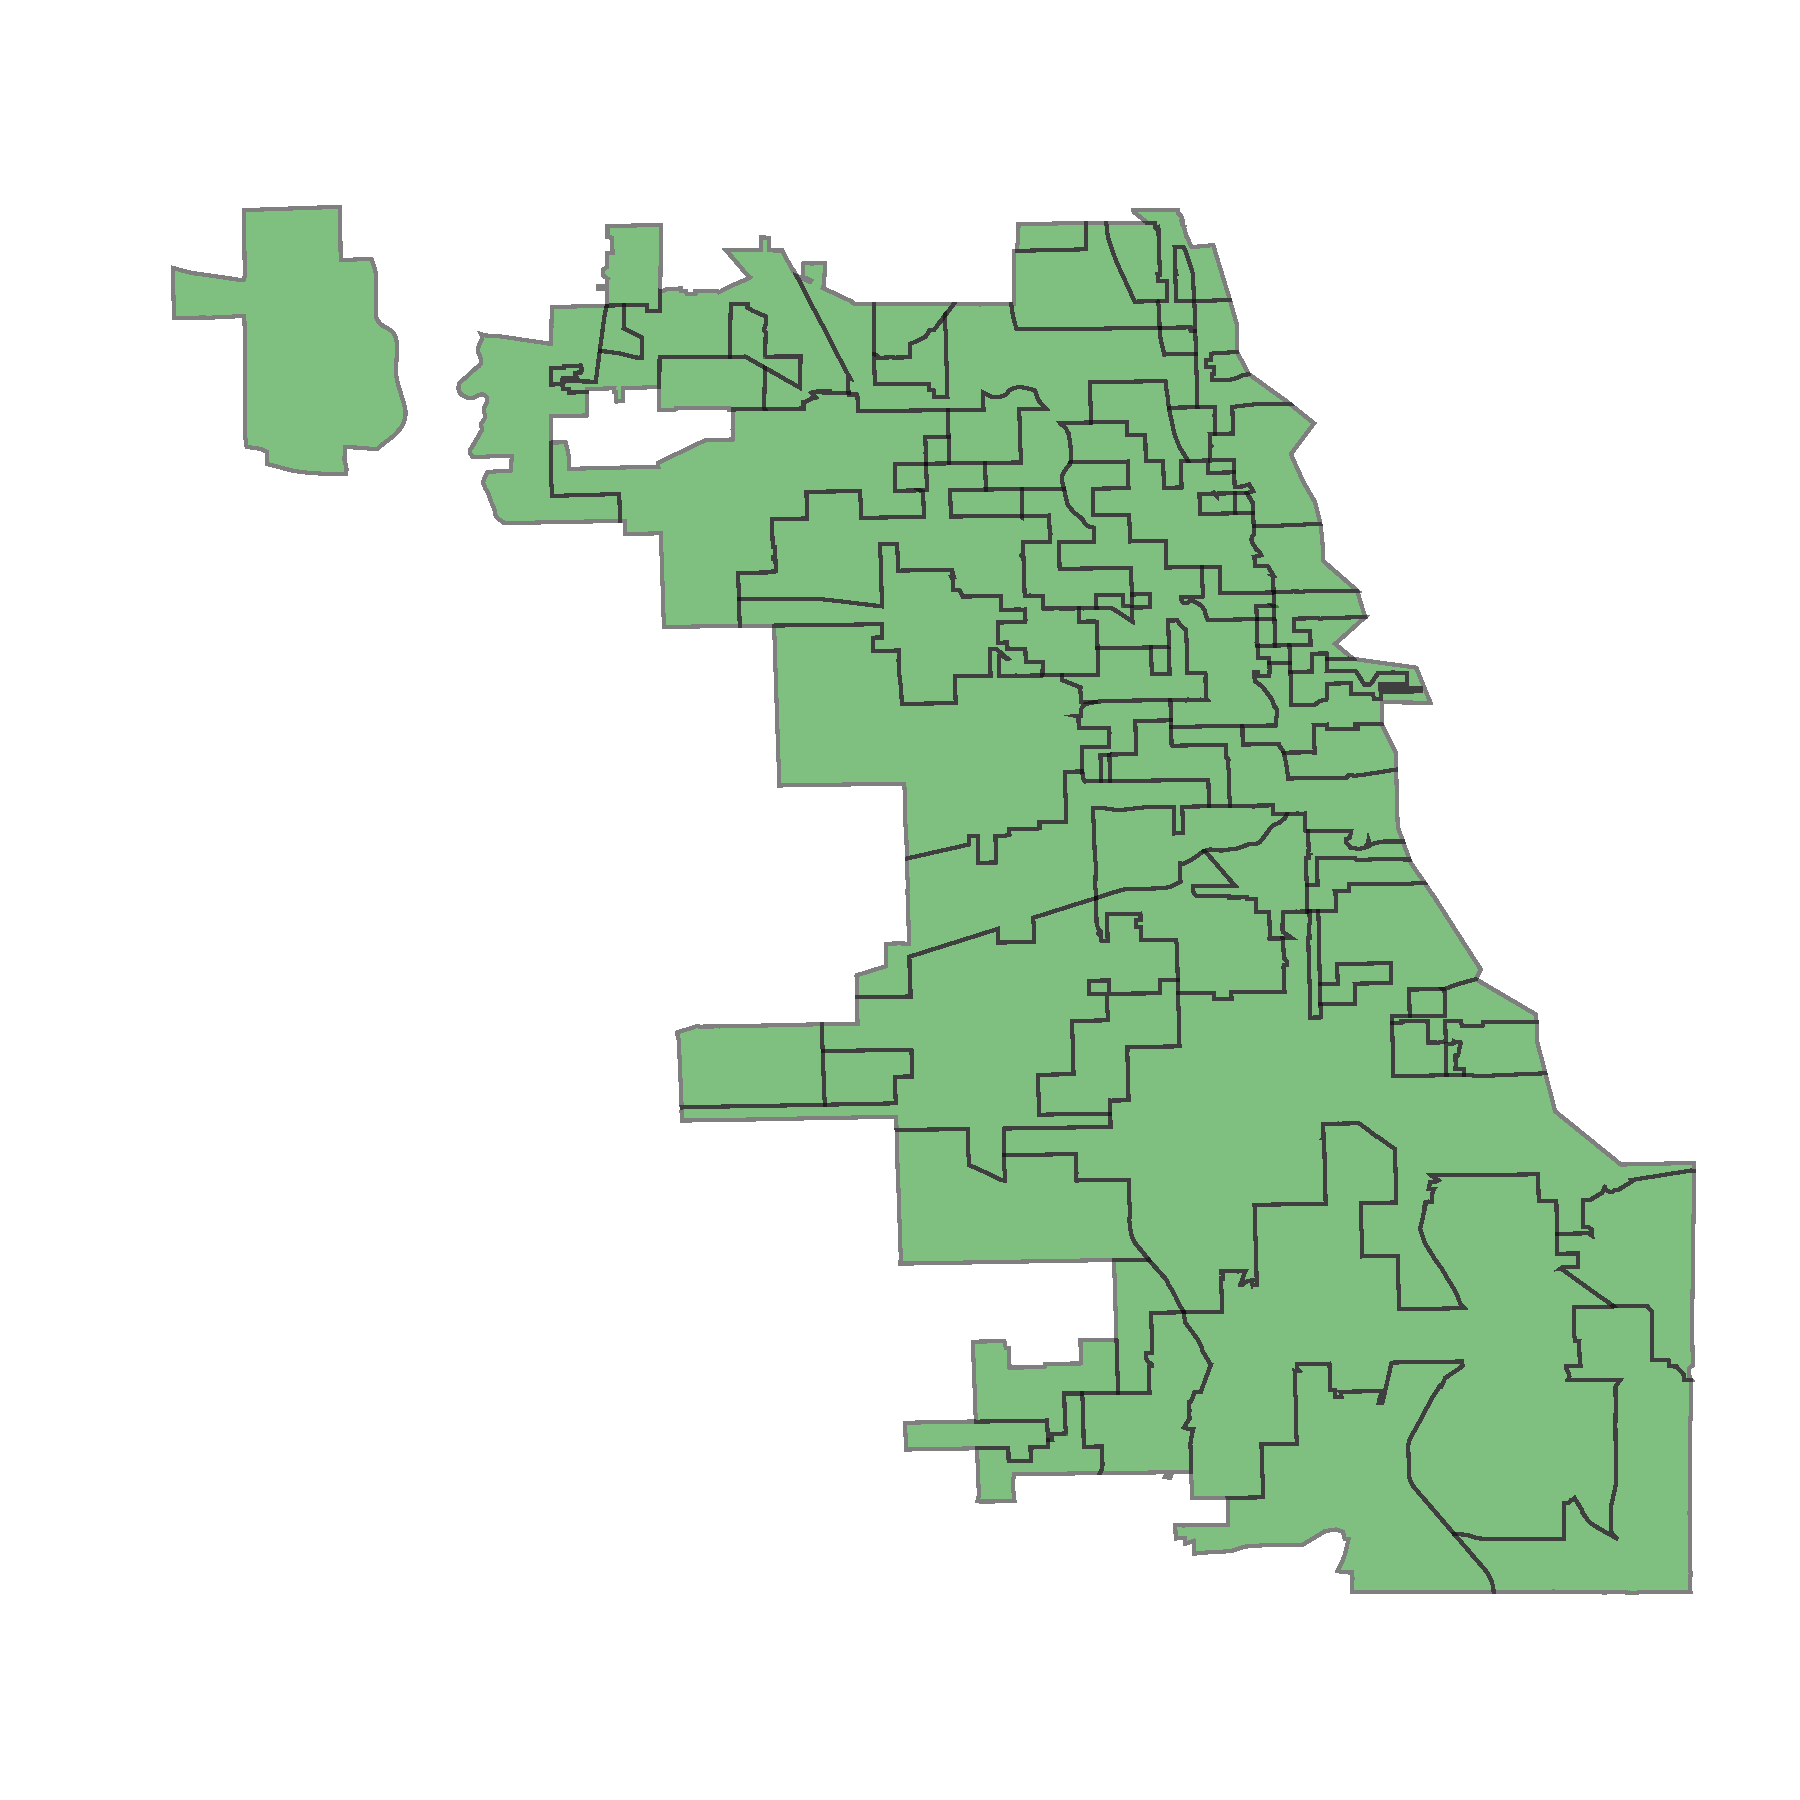
\includegraphics[width=0.45\linewidth]{fig/agg_CAs.pdf}}
\subfigure[\texttt{K-Means}]{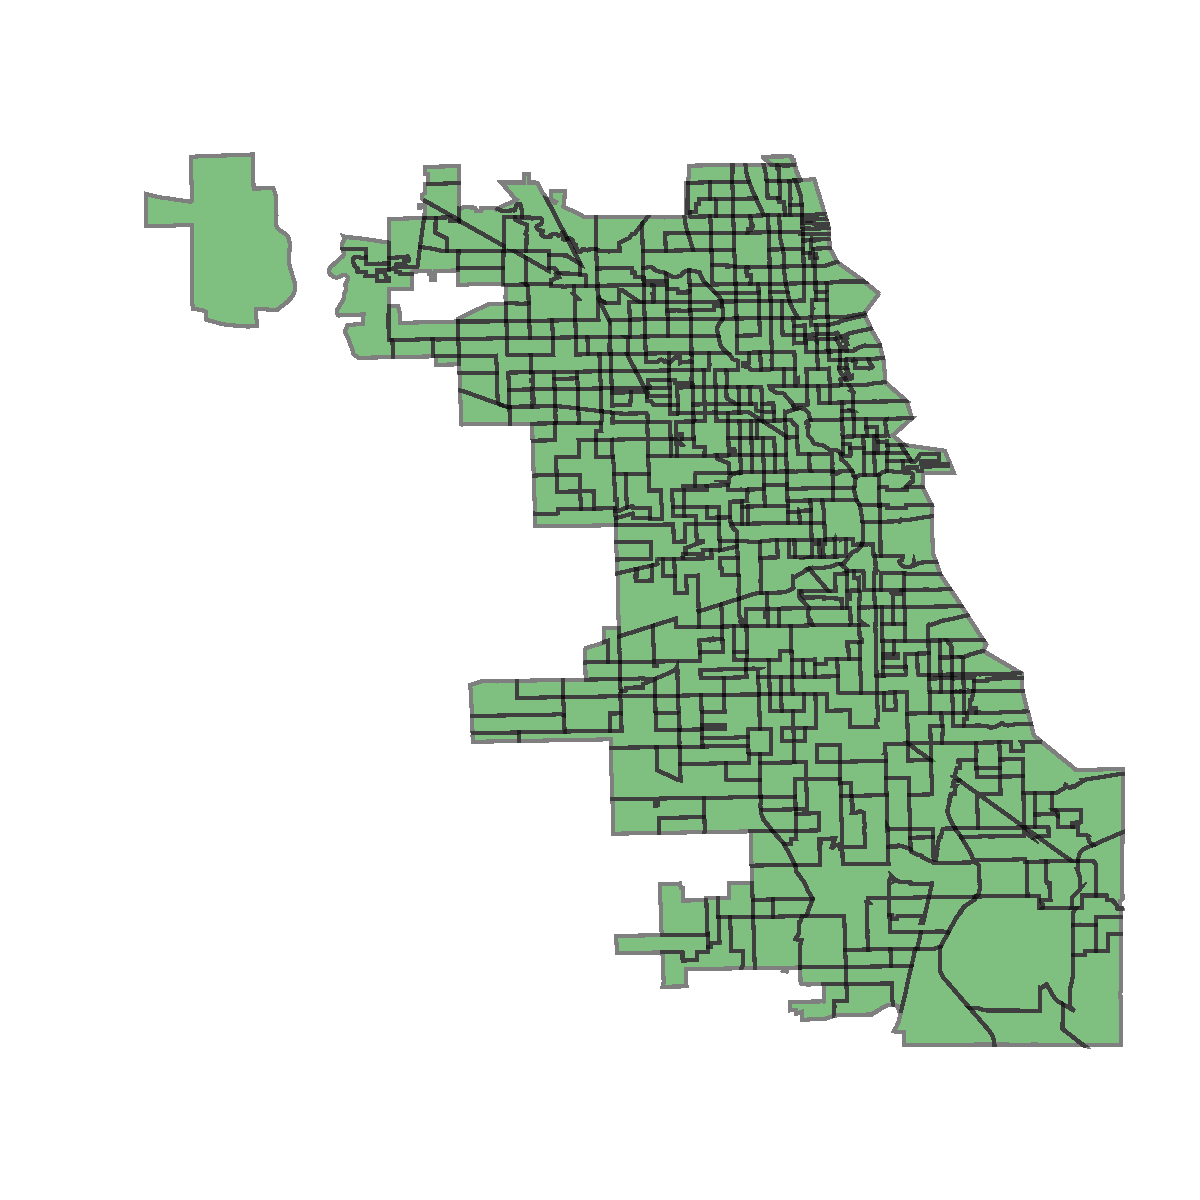
\includegraphics[width=0.45\linewidth]{fig/kmeans_CAs.pdf}}
\subfigure[\texttt{Spectral}]{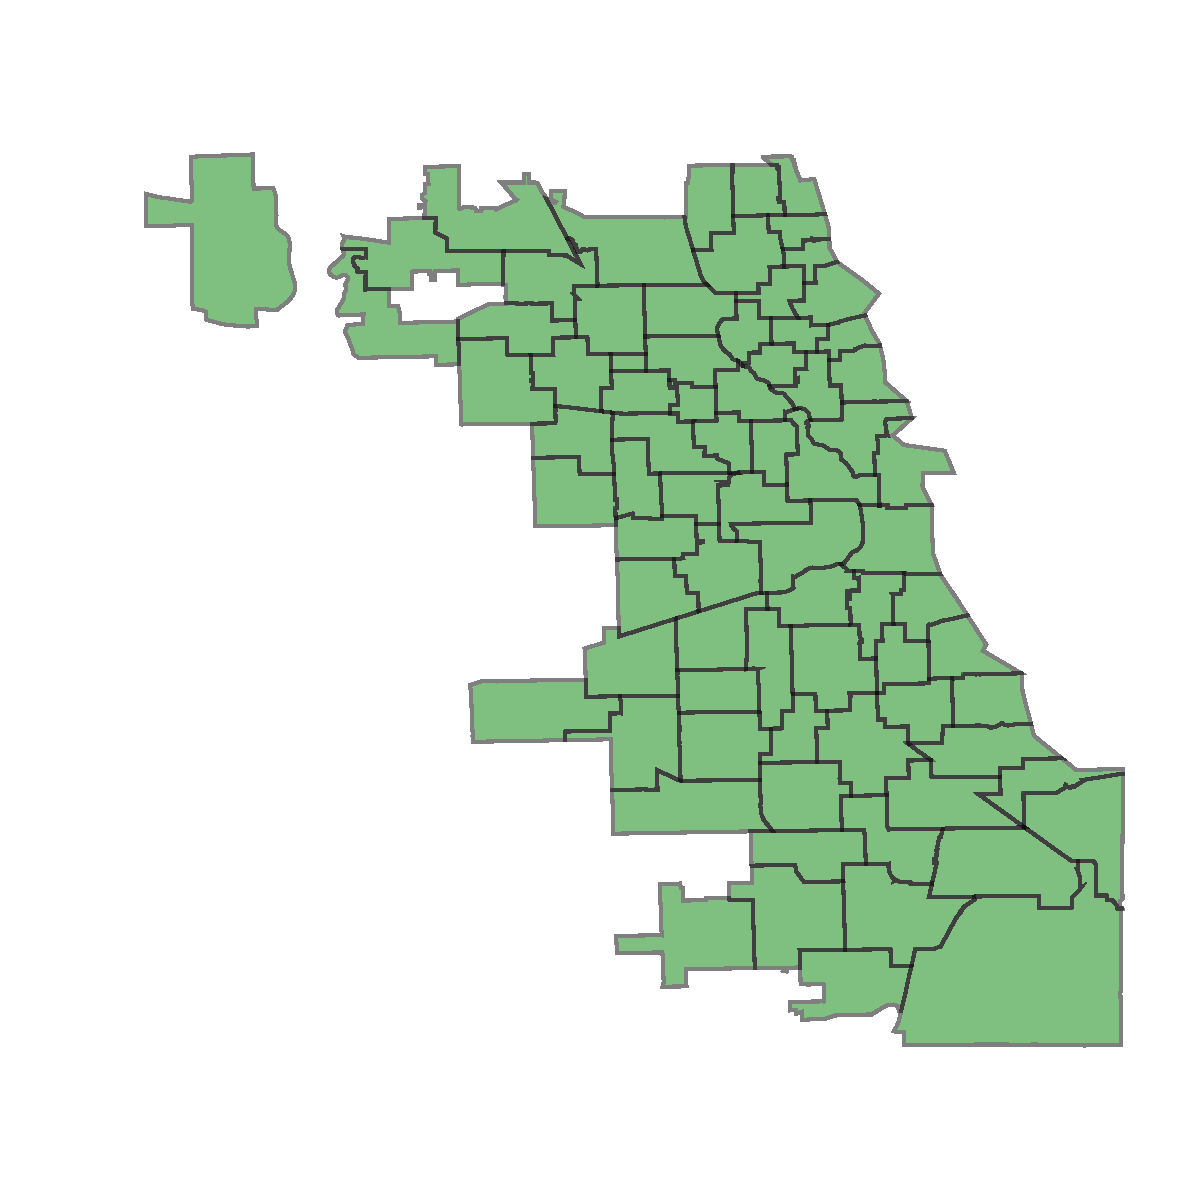
\includegraphics[width=0.45\linewidth]{fig/spectral_CAs.pdf}}
\subfigure[\texttt{DQN}]{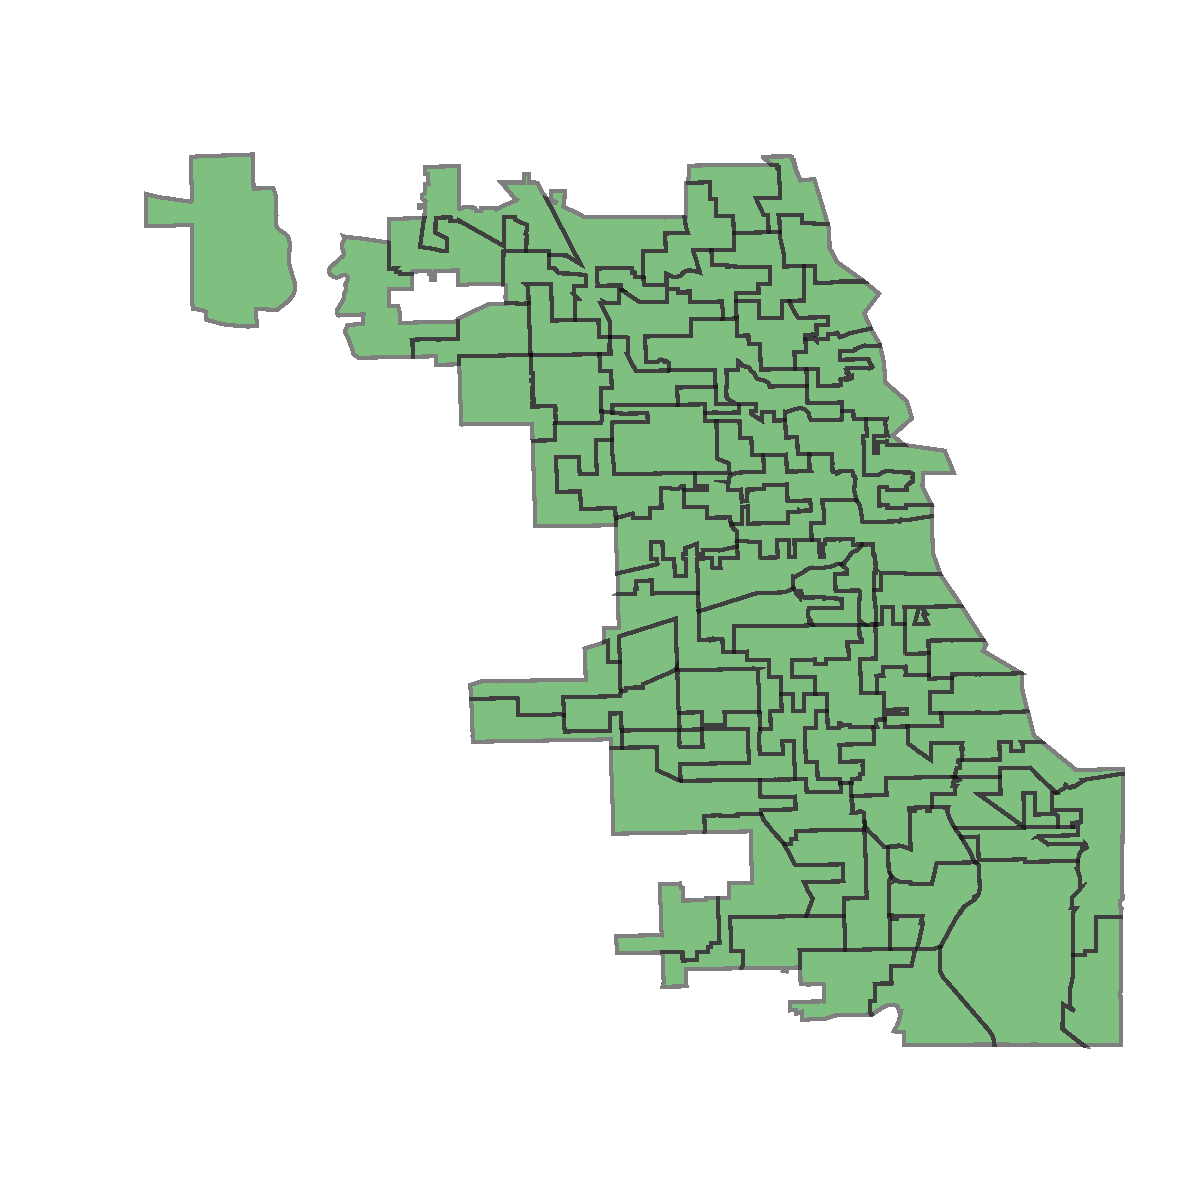
\includegraphics[width=0.45\linewidth]{fig/case-study-house-price-q-learning-v10-CAs.pdf}}
\caption{(a - c) The clustering results for three clustering baselines. (d) The learned partition from \texttt{DQN} method for crime prediction task.}
\label{fig:partitions}
\end{figure*}



\begin{itemize}[leftmargin=*]
\item \textbf{(\texttt{Admin})} Administrative boundary  uses the existing administrative boundary defined by US Bureau of Census~\cite{census:2010}. A visual depiction of this partition can be seen in Figure~\ref{fig:intro}. %This baseline partition is denoted as \texttt{Admin}. 
\item \textbf{(\texttt{Agglomerative})} Agglomerative clustering performs a hierarchical clustering using a bottom up approach. The ward linkage function is used, along with a tract adjacency graph as input to guarantee spatial continuity. %This method is denoted as \texttt{Agglomerative}.
\item \textbf{(\texttt{K-Means})} K-means clustering separates tracts into $n$ groups of equal variance.%, denoted as \texttt{K-Means}.
\item \textbf{ (\texttt{Spectral})} Spectral clustering does a low-dimensional embedding of the affinity matrix between samples first, and then applies the K-means method in the lower dimensional space. Note that \texttt{Spectral} also takes the tract adjacency graph as the affinity graph.
\item \textbf{(\texttt{Naive})} MCMC with naive proposal. The first variant of our proposed MCMC method using a straightforward uniform proposal.
\item \textbf{(\texttt{Softmax})} MCMC with softmax proposal is another variant of our MCMC method, which uses strong heuristics.
\item \textbf{(\texttt{DQN})} Q-learning is our proposed reinforcement learning method to search for optimal partition.
\end{itemize}

For various clustering methods, we set the number of clusters as $m=77$, which equals the number of community areas in \texttt{Admin}. Note that if we run clustering methods multiple times, they usually produce the exact same clustering results. The MCMC and \texttt{DQN} methods, on the other hand, are all stochastic processes and do not converge to the same partition. Therefore, we run $100$ rounds of our proposed methods and report the average measure.



\subsubsection{Evaluation Metrics} 


Given a partition $\mathcal{Z}$, we evaluate the quality of this partition on the testing data set.
Mean absolute error (MAE) is used to measure the performance of prediction tasks, i.e.
\begin{equation}
MAE = \frac{ \sum_{j=1}^m |Y_j - \hat{Y_j}| }{ m},
\end{equation}
where $\hat{Y_i}$ is the leave-one-out prediction error of community $Z_j$. Namely, we train a model on the rest of the communities $\mathcal{Z} \setminus Z_j$. Then, $\hat{Y_j}$ is the estimated target value for $Z_j$ from the trained model.


\subsection{Quantitative Evaluations}

\subsubsection{Effectiveness Study}

In Table~\ref{tab:mae}, we report the evaluation results of the various partition methods. The partitions results from different baselines are visualized in Figure~\ref{fig:partitions}(a-c). Since our methods are run for 100 rounds, we report both the MAE and its standard deviation in the table. The final partition of \texttt{DQN} is visualized in Figure~\ref{fig:partitions}(d). Overall, we have the following three observations.


\begin{table}[h!]
\centering
\caption{Prediction MAEs of various partition methods. Our proposed methods are run for 100 rounds. The MAE and its variance are reported.}
\label{tab:mae}
\begin{tabular}{ |c|>{\raggedleft\arraybackslash}p{4cm}|>{\raggedleft\arraybackslash}p{4cm}|} 
\hline
 Method & \multicolumn{2}{c|}{MAE}  \\ \hline
   & Crime & House price \\
 \hline
 \texttt{Admin} & 1715.91 & 31.29  \\ 
 \hline
 \texttt{Agglomerative} & 72201.00 & 50.34 \\
 \hline
 \texttt{K-means} & 2887.83 & 32.40 \\
 \hline
 \texttt{Spectral} & 1440.57 & 29.66  \\
 \hline
 \texttt{Naive} & 1073.42(81.93) & 25.73(2.76) \\
 \hline
 \texttt{Softmax} & 1041.68(76.75) & 27.13(2.98) \\
 \hline
 \texttt{DQN} & \textbf{746.13}(154.19) & \textbf{25.16}(1.30) \\
 \hline
\end{tabular}
\end{table}


\emph{Clustering methods overall perform poorly}. This is likely due to the fact that the clustering methods do not consider the task information. More specifically, \texttt{Agglomerative} results in the highest prediction errors for both crime prediction and house price prediction task. The reason is that  \texttt{Agglomerative} method utilizes tract connectivity as a hard constraint. As a result, the generated communities have a large variance in their sizes, as shown in Figure~\ref{fig:partitions}(a).  \texttt{K-Means} gives worse result than that of \texttt{Admin} as well. The generated partition of \texttt{K-Means} seems to consist of more than $m$ communities in Figure~\ref{fig:partitions}(b) because \texttt{K-Means} does not incorporate spatial continuity constraint. Consequently, one community can consist of several disconnected components.  \texttt{Spectral} methods generates the best results in both tasks among these baselines because \texttt{Spectral} accounts for the affinity of tracts and generates communities with similar sizes. However, it is worth mentioning that  \texttt{Spectral} method cannot guarantee the spatial continuity of generated communities. From Figure~\ref{fig:partitions}(c), we can also see that \texttt{Spectral} shows similar partition as the original administrative boundary, shown in Figure~\ref{fig:intro}(a). That is also why it achieves similar prediction accuracy as \texttt{Admin}.



\emph{The proposed MCMC method outperforms the baselines}. Both variants of MCMC methods significantly outperform  \texttt{Admin} and \texttt{Spectral} baselines. Such observations validate the effectiveness of the MCMC strategy in searching for optimal solutions. However, it is not conclusive to say \texttt{Softmax} is better than \texttt{Naive}, because while \texttt{Softmax} has better performance on crime prediction task,  \texttt{Naive} has better performance in house price prediction. The reason could be that the heuristics used in \texttt{Softmax} is not universally applicable. The heuristic assumes that working on a community with the highest error will lead to optimal solution. When this heuristic is wrong, it aggressively reduces the search space, excluding where there are better local optimal partitions. 



\emph{ \texttt{DQN} method performs the best among all}. It is clear that  \texttt{DQN} finds a better local optimal solution than that of MCMC methods. On the crime prediction task, the average MAE is $746.13$, which represents a $56\%$ improvement over  \texttt{Admin} baseline. On the house price prediction task, \texttt{DQN} consistently gives the best performance. The reason is that \texttt{DQN} explores over a subset of actions and picks the best one at each step, compared to the MCMC method, which searches the partition space in a depth first search fashion. Comparing the final partition of \texttt{DQN} and \texttt{Spectral}, we will notice that \texttt{Spectral} partition is more similar to the original administrative boundary in Figure~\ref{fig:intro}. As a consequence,  \texttt{Spectral} has similar MAE to \texttt{Admin}, but is much worse than \texttt{DQN}.


\begin{figure}[t!]
\centering
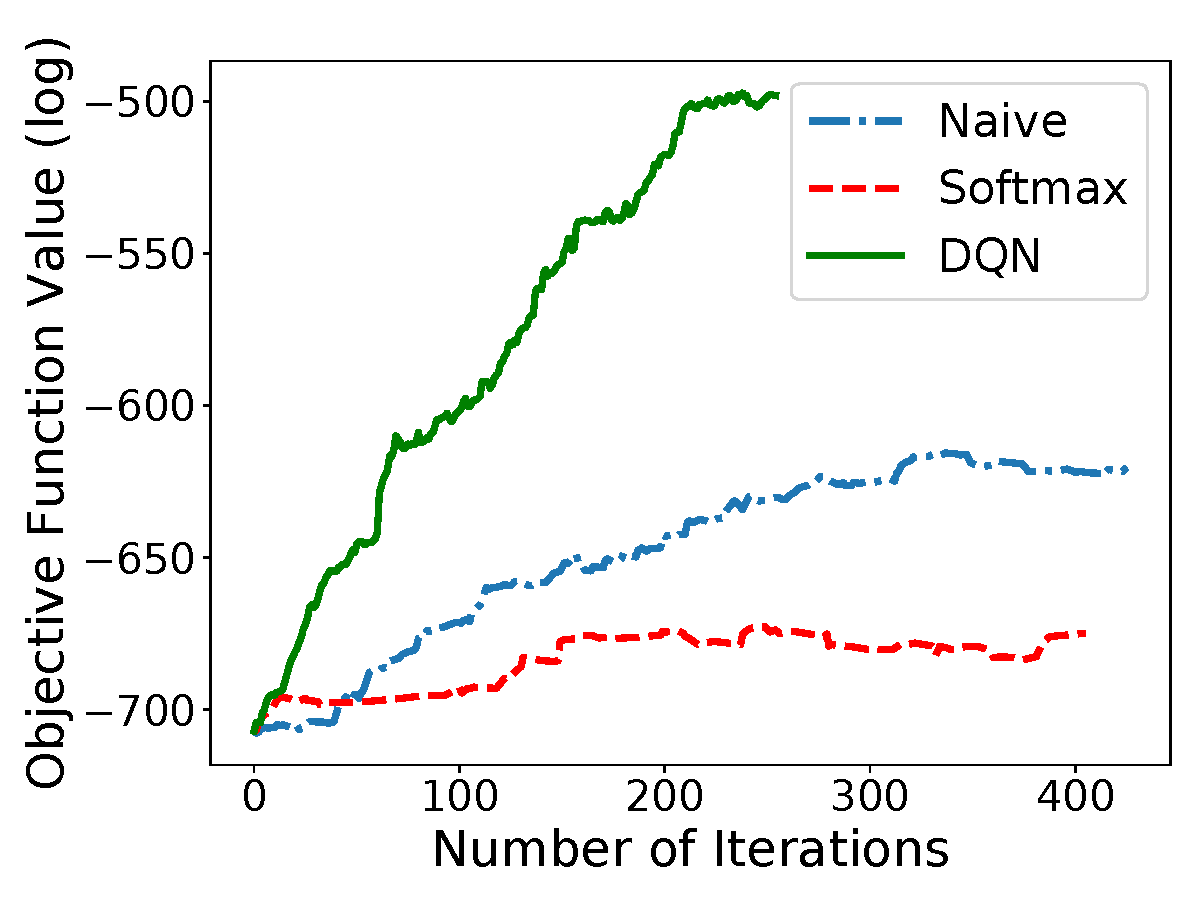
\includegraphics[width=0.9\linewidth]{fig/convergence-study.pdf}
\caption{Convergence plots for proposed methods on house price prediction task.}
\label{fig:convergence}
\end{figure}



\begin{figure*}[t!]
\centering
\subfigure[All communities]{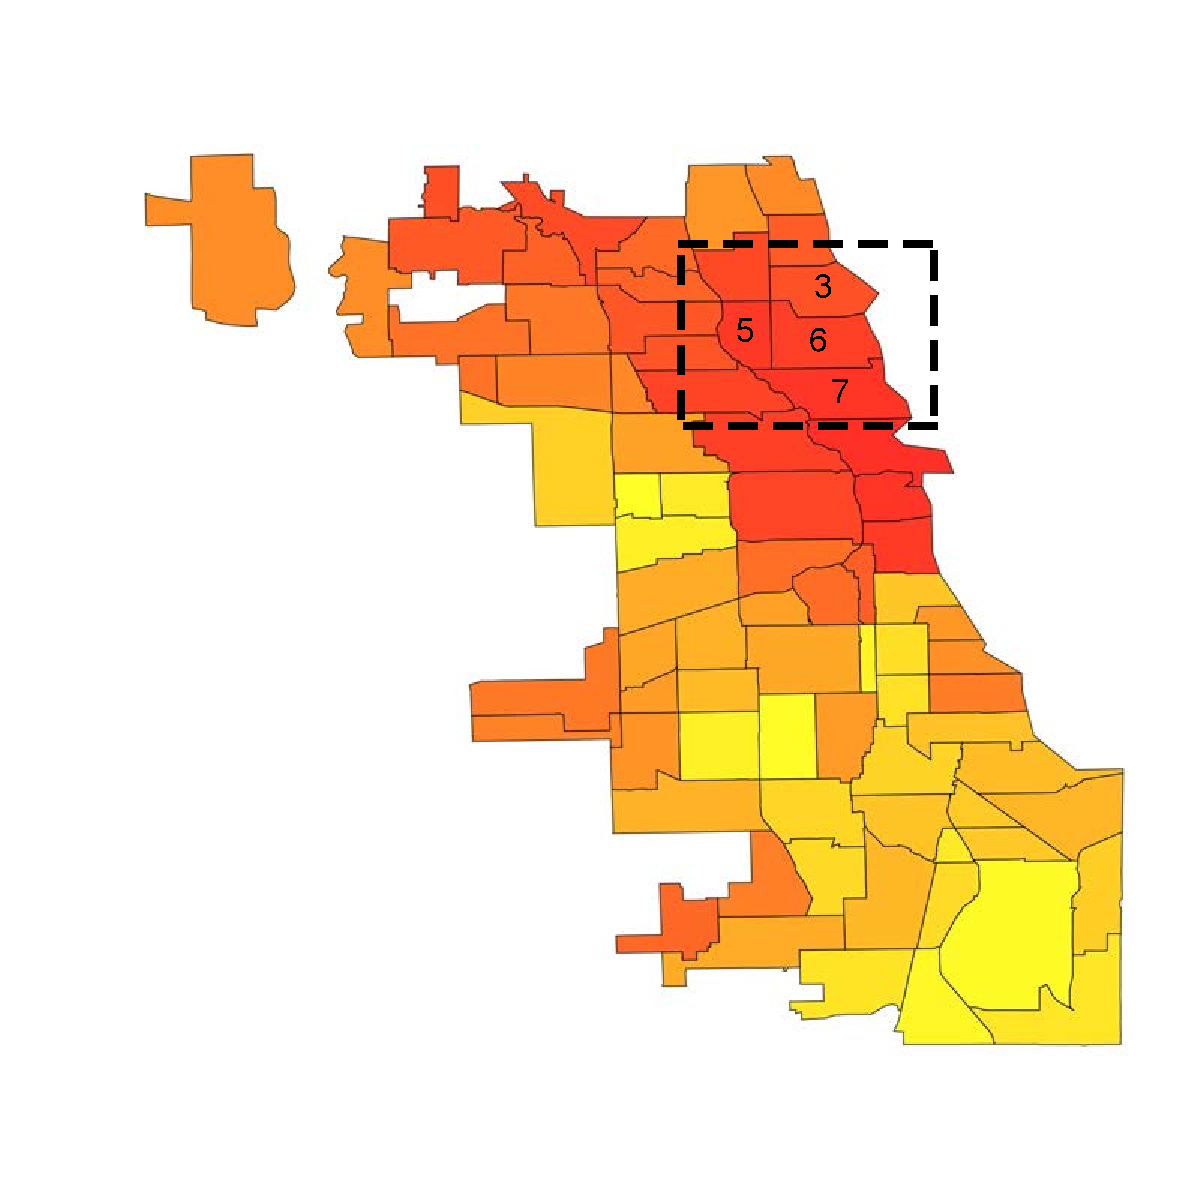
\includegraphics[width=0.3\linewidth]{fig/before-train_average_house_price-all-final.pdf}}
\subfigure[Before]{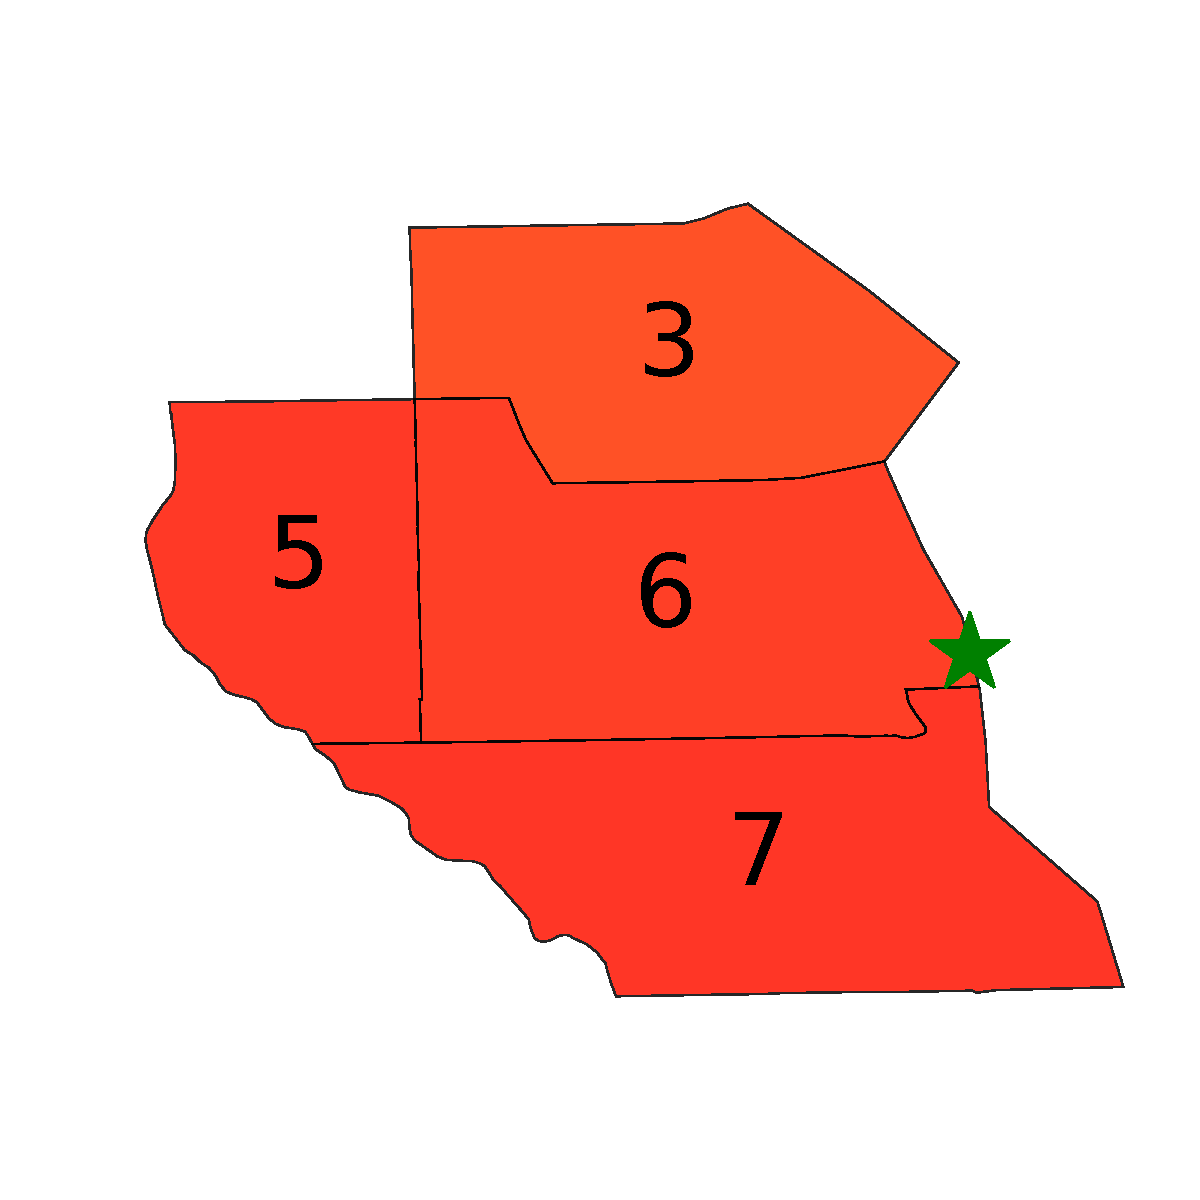
\includegraphics[width=0.28\linewidth]{fig/before-train_average_house_price.pdf}}
\subfigure[After]{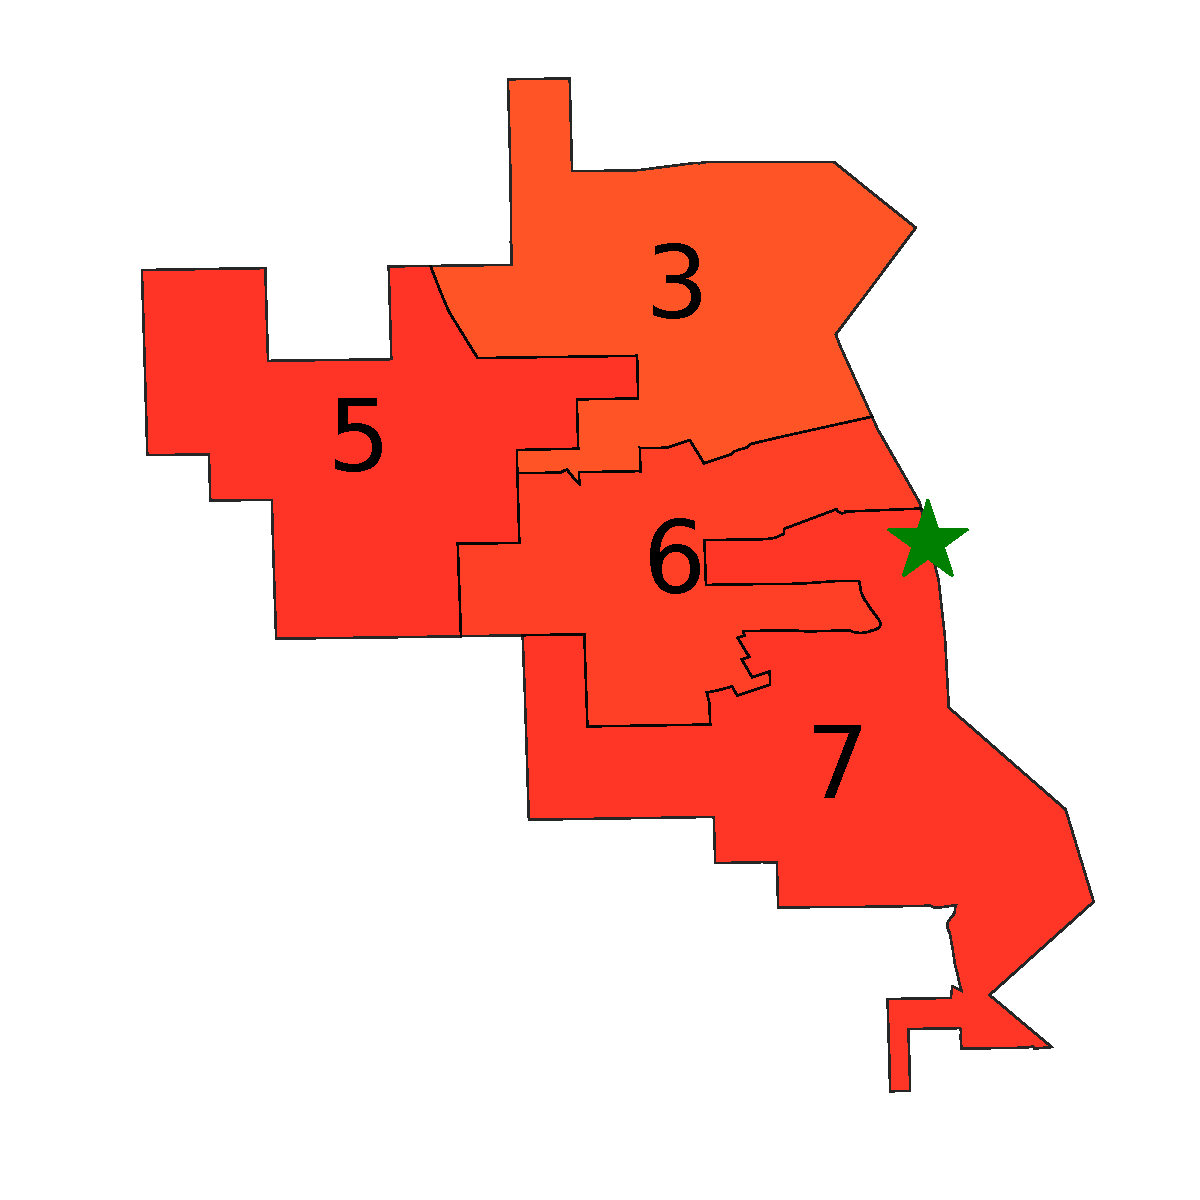
\includegraphics[width=0.3\linewidth]{fig/after-train_average_house_price.pdf}}
\subfigure[Lake View]{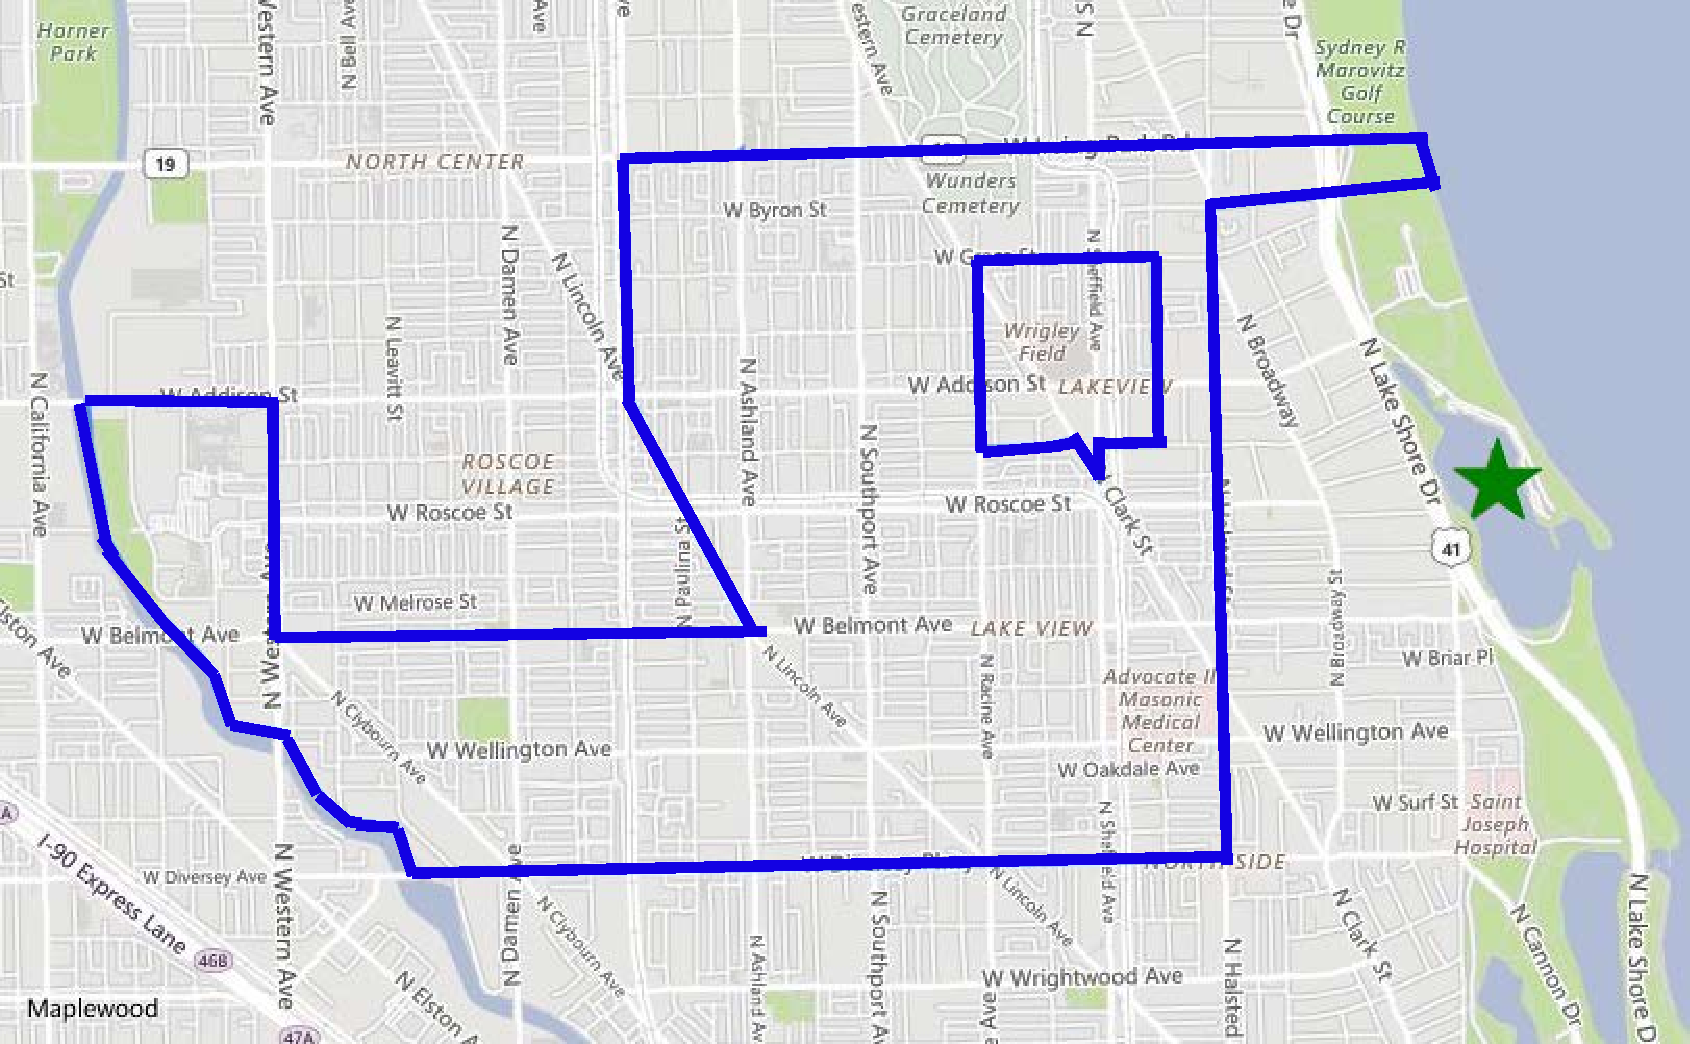
\includegraphics[width=0.45\linewidth]{fig/ca-lakeview.pdf}}
\subfigure[Lake View East]{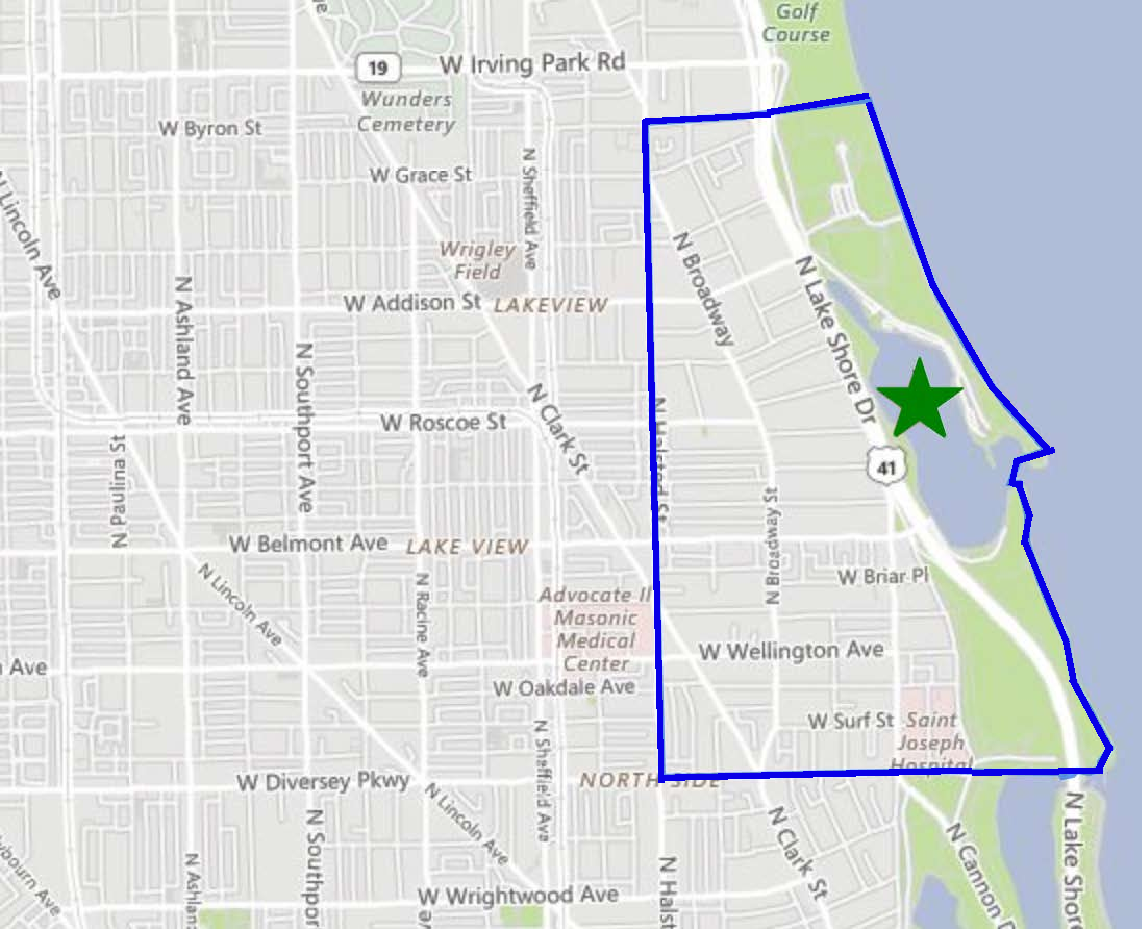
\includegraphics[width=0.34\linewidth]{fig/ca-lakeview-east.pdf}}
\caption{House price prediction case near Belmont Harbor, denoted by green star. (a) Average house price distribution in Chicago under \texttt{Admin} partition. Dotted rectangle denotes region of interest. (b) Region of interest under \texttt{Admin} partition. (c) Region of interest under \texttt{DQN} partition. (d - e) Region of interest according to Zillow. Note that the Belmont Harbor area is split into a separate community, named Lake View East.}
\label{fig:housePrice}
\end{figure*}



\subsubsection{Convergence Study}

We conclude the effectiveness study with a brief comparison of the convergence of three proposed methods. In our method, we track the standard deviation of the $\mathcal{F}$ values from last $50$ iterations. When such standard deviation is less than a pre-defined threshold, we stop. In Figure~\ref{fig:convergence} we visualize log of quality measure, i.e. $ - \mathcal{F}(\mathcal{Z})$, against the number of iterations for three proposed methods on the house price task. 

We observe that \texttt{DQN} finishes in a less than 300 iterations, while \texttt{Naive} and \texttt{Softmax} both take more than 400 iterations. Clearly, we observe that \texttt{DQN} converge to a better optimal solution with higher training gain. Comparing with \texttt{Naive},  \texttt{Softmax} converges faster at the beginning, because of the strong heuristics behind. However, \texttt{Naive} eventually finds a better local optimal solution than that of \texttt{Softmax}, because the heuristics eliminates search space too aggressively, such that the algorithm could not explore search space with better local optimal partitions.









\subsection{Case Studies}

In this section, we present two interesting case studies of the region partitions learned from \texttt{DQN} method.

\smallskip
\textbf{House price prediction case study}. We present a case study near community \#6, Lake View, in the house price prediction task, as shown in Figure~\ref{fig:housePrice}. This case shows that \texttt{DQN} partition is actually superior to the original administrative boundary, because  \texttt{DQN} partition matches better with expert domain knowledge.

We visualize a heat map of house price (per square foot) for the whole city of Chicago in Figure~\ref{fig:housePrice}(a). Warmer colors (red) denote higher prices, while cooler colors (yellow) indicate lower prices. The dotted rectangle in the figure marks the region of interest for our discussion, which is community \#6. A zoom-in view of this area using the administrative boundary is shown in Figure~\ref{fig:housePrice}(b). Notice that all nearby areas have relatively high average house price.


Recall from the Figure~\ref{fig:intro-explain} that east side of community \#6 is different from the rest area of community \#6. We further find the following evidence to support the fact that the east side of community \#6 is different from the rest area. The coastal region of the original community \#6 contains Belmont Harbor, one of Chicago's largest boating areas. Notice that  \texttt{DQN} method divides community area \#6 and groups the coastal tracts surrounding the Belmont Harbor with other coastal areas farther south in community \#7. These areas contain other leisure destinations such as the Lincoln Park Zoo, and numerous beach areas. This semantic argument is bolstered by an independent source: Zillow's own self-defined regions. Figure~\ref{fig:housePrice}(d) shows that the Lake View area does not contain Belmont Harbor. Meanwhile, Zillow assigns Belmont Harbor as a separate region called Lake View East, as shown in Figure~\ref{fig:housePrice}(e). 


Surprisingly,  \texttt{DQN} partition is similar to Zillow's self-defined region in that they both exclude the Belmont Harbor area from the original community \#6 (Lake View neighborhood), as shown in Figure~\ref{fig:housePrice}(c). While the two regions are not exactly the same, it is interesting to note that they both remove the Belmont Harbor area from the original community.



\begin{figure*}[t!]
\centering
\subfigure[All communities]{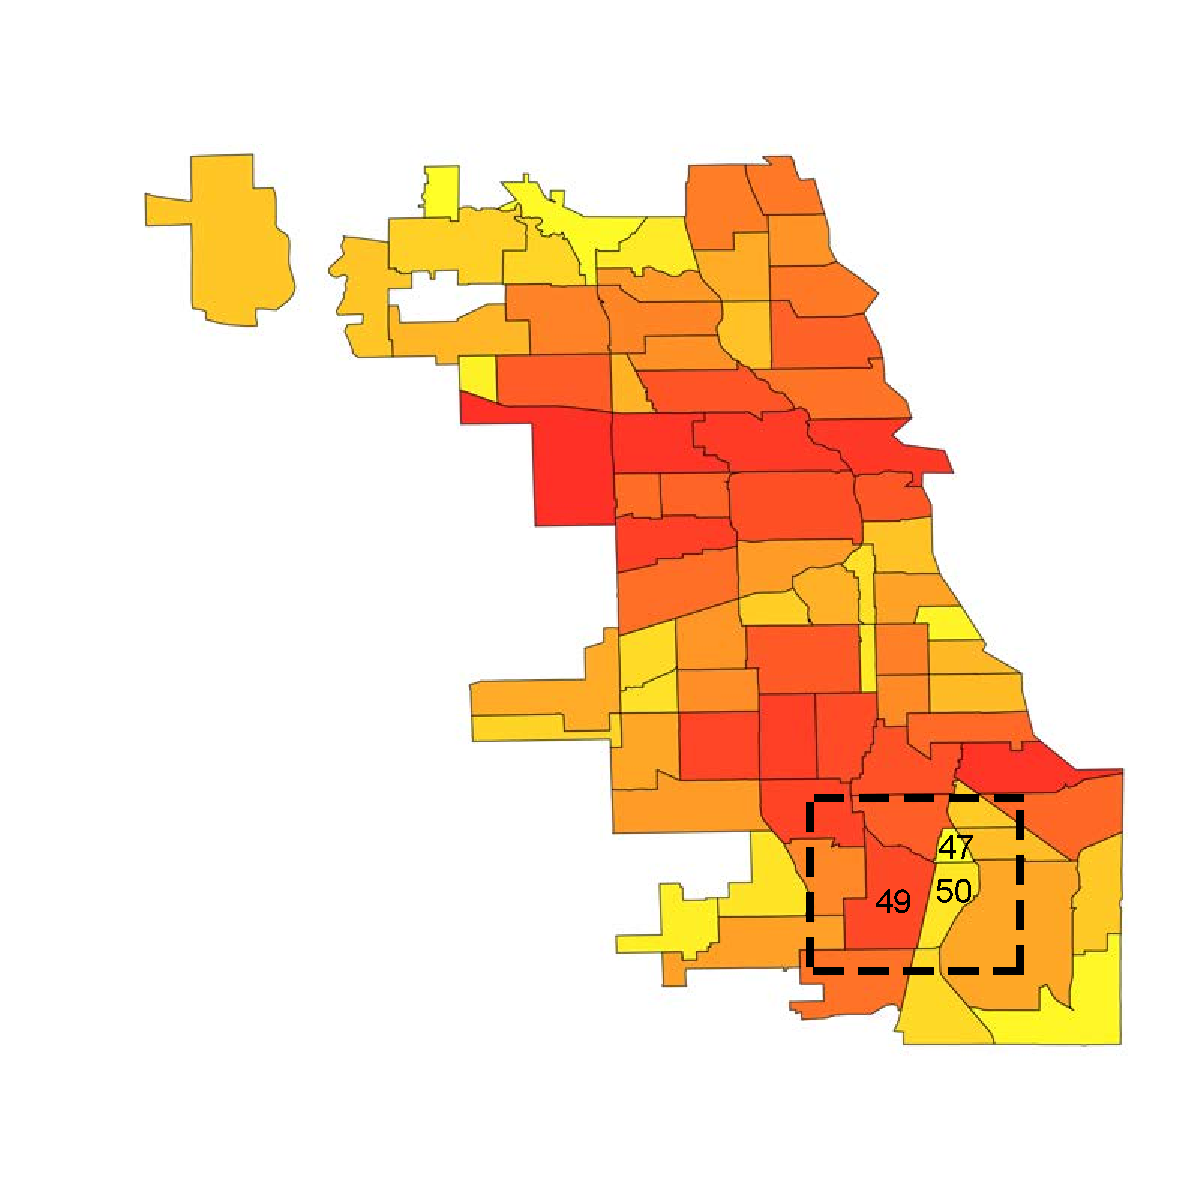
\includegraphics[width=0.3\linewidth]{fig/before-total-all-final.pdf}}
\subfigure[Crime Before]{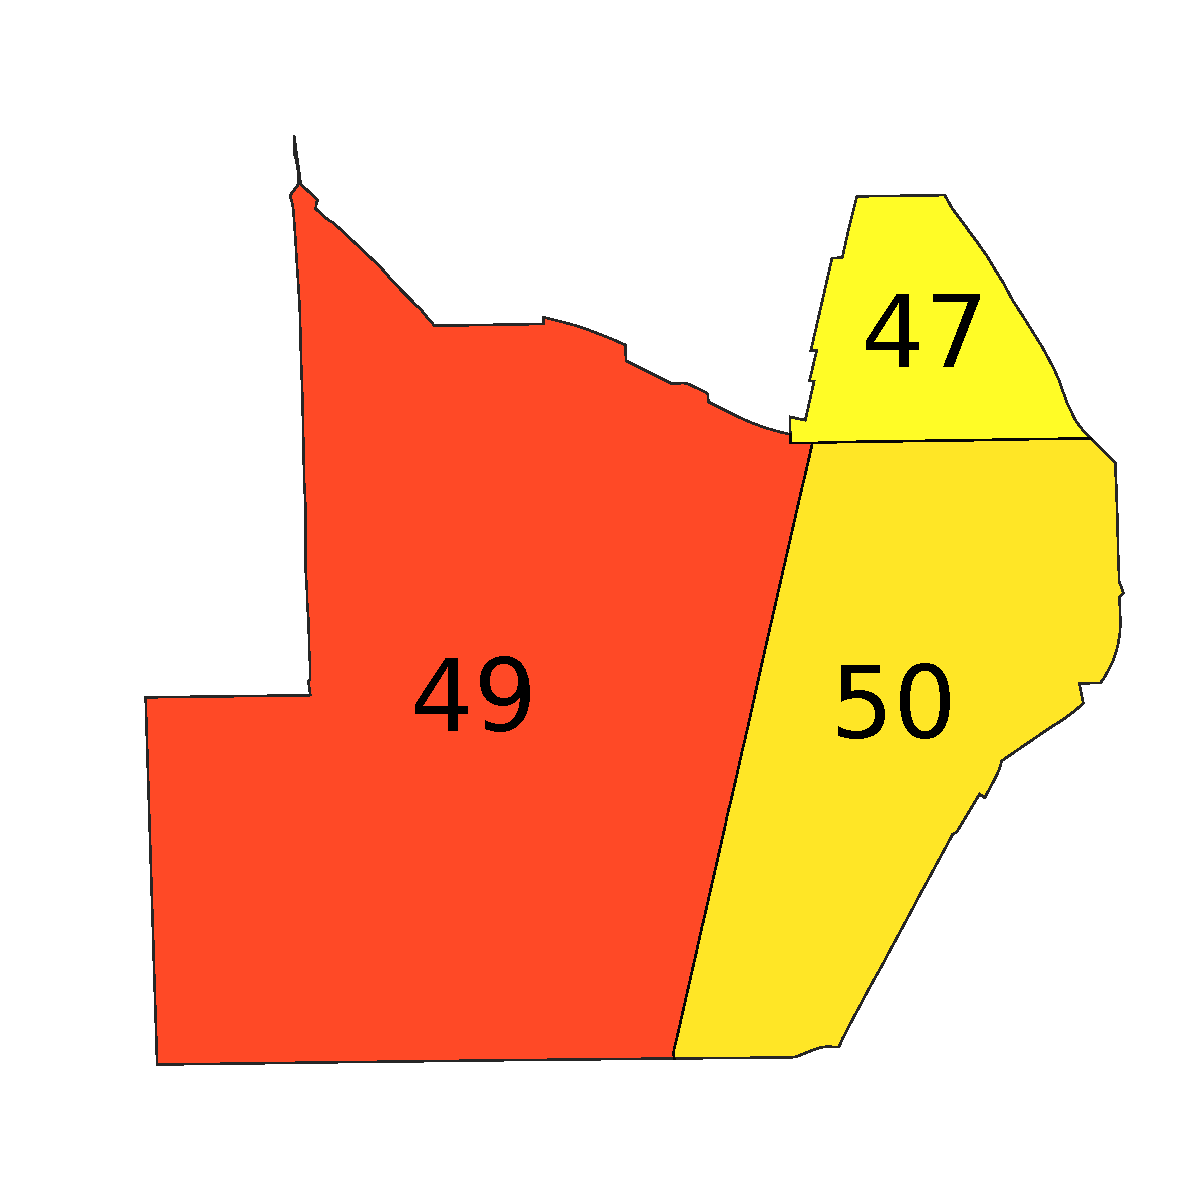
\includegraphics[width=0.28\linewidth]{fig/before-total.pdf}}
\subfigure[Poverty Before]{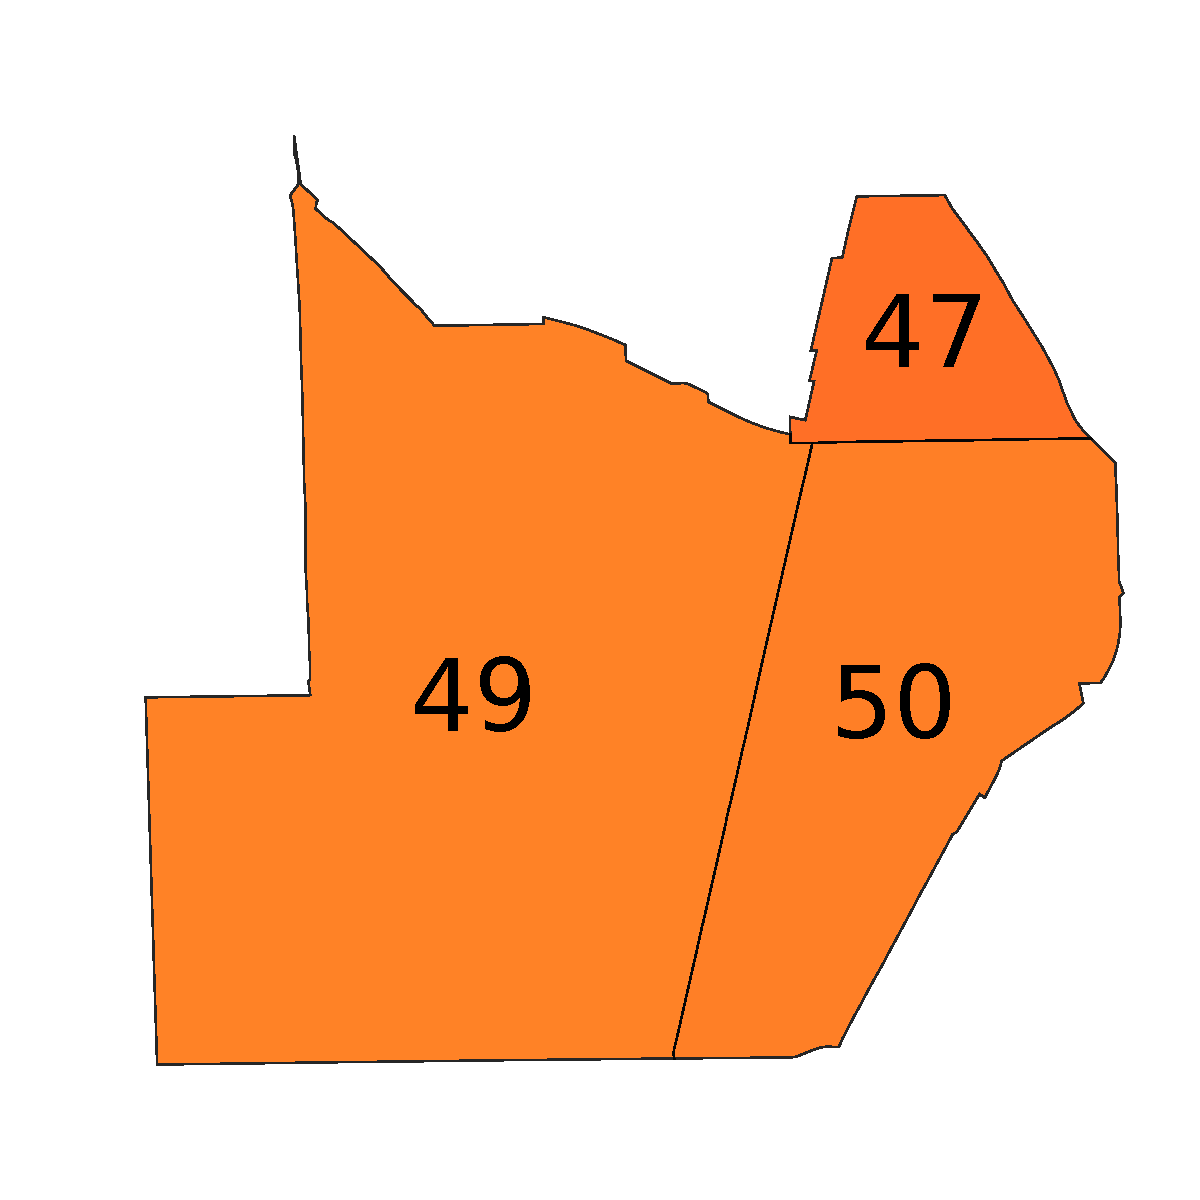
\includegraphics[width=0.28\linewidth]{fig/before-poverty_index.pdf}}
\subfigure[Crime After]{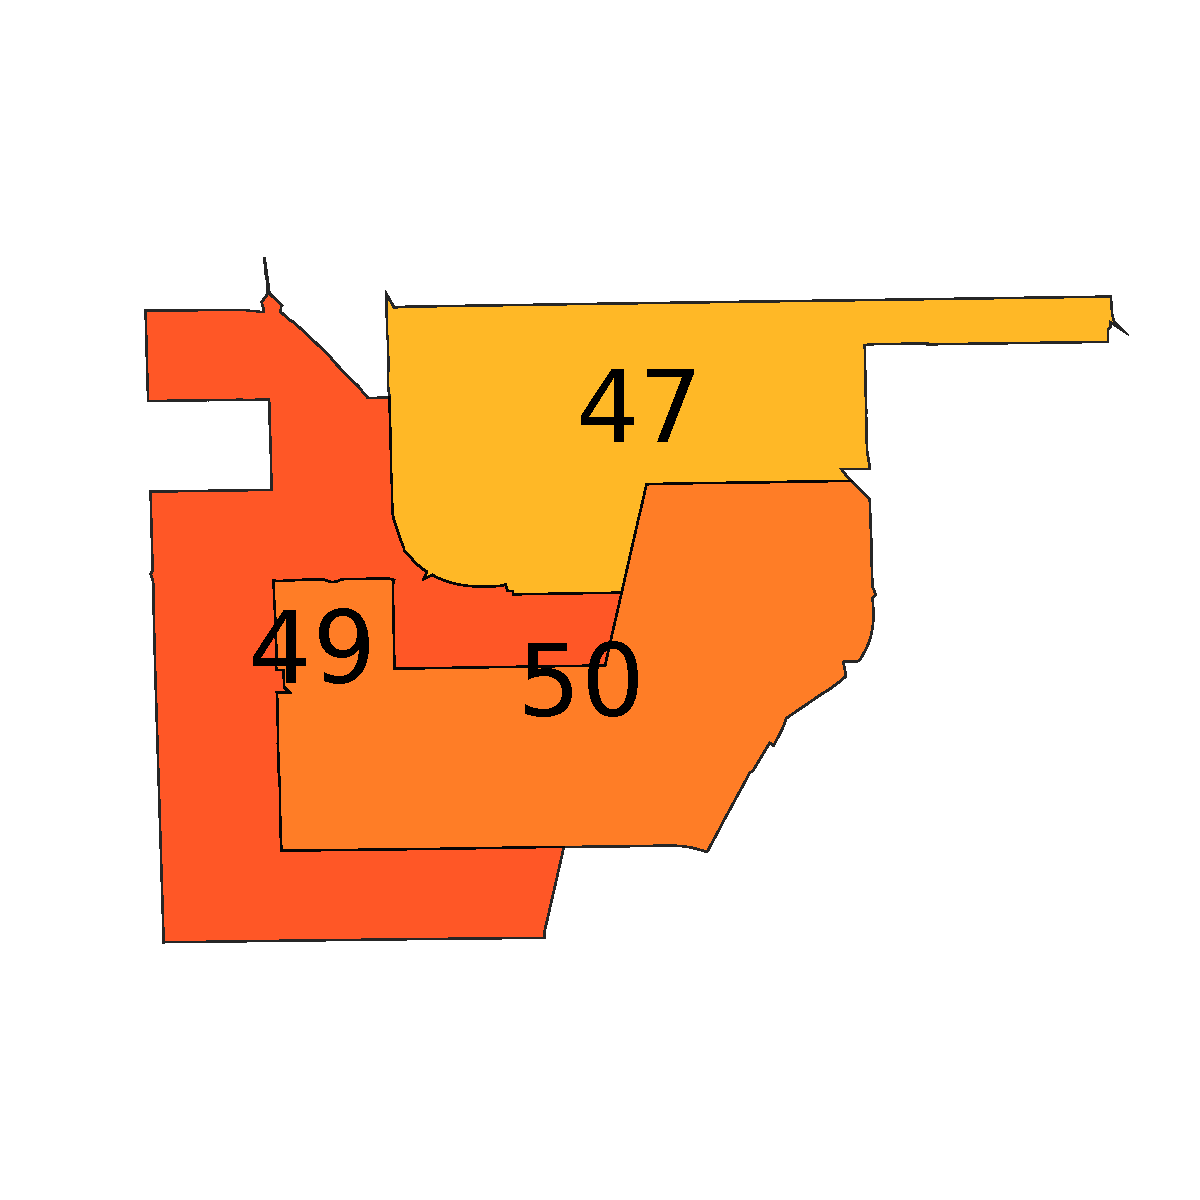
\includegraphics[width=0.32\linewidth]{fig/after-total.pdf}}
\subfigure[Poverty After]{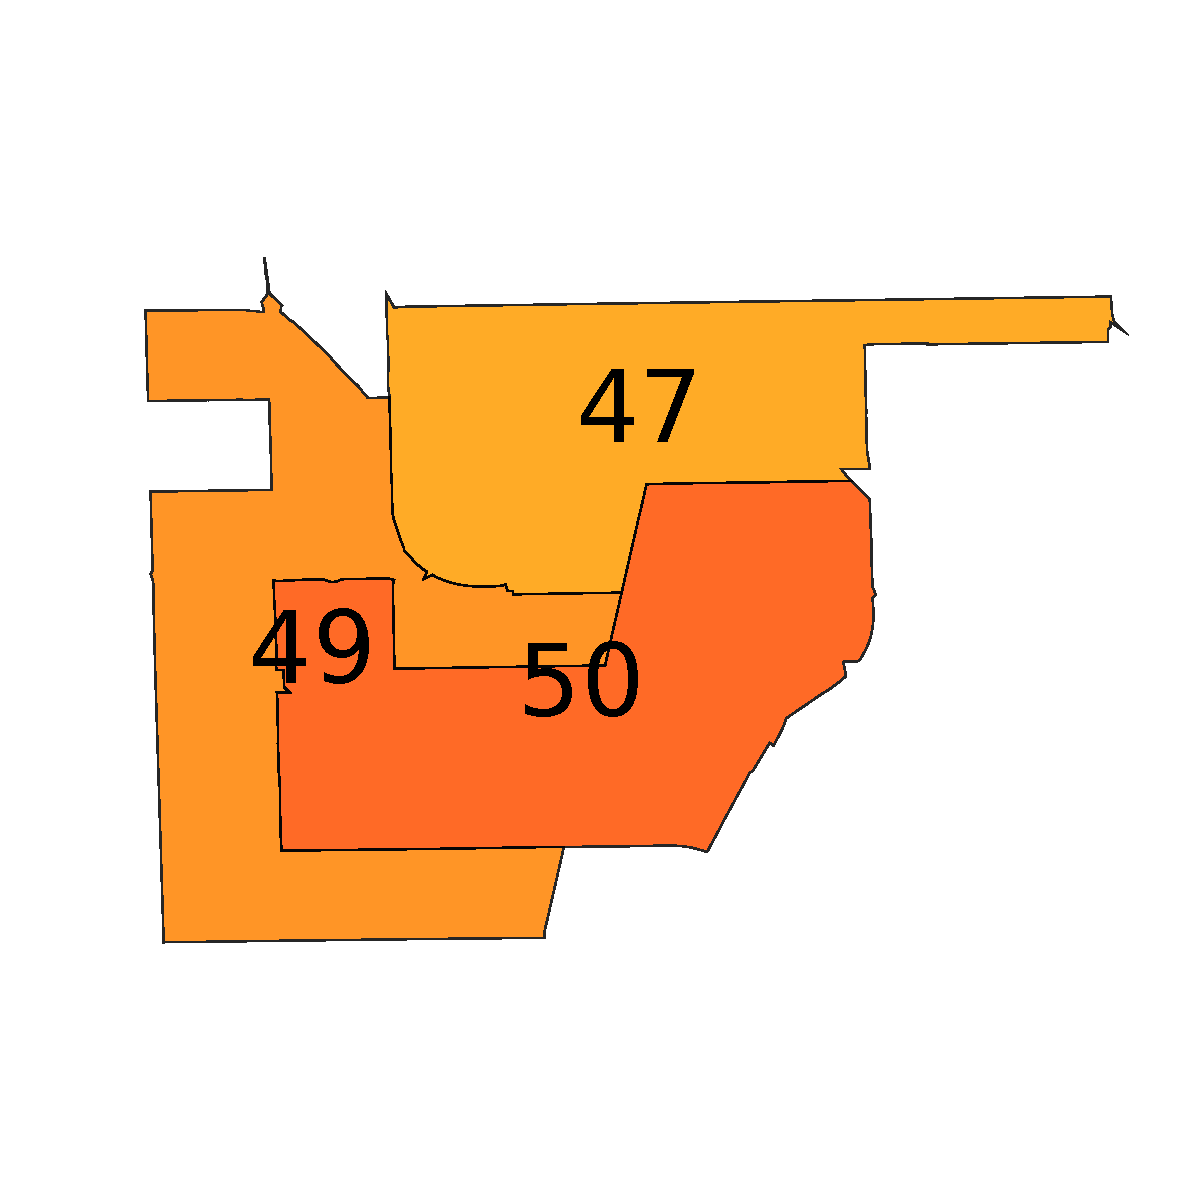
\includegraphics[width=0.32\linewidth]{fig/after-poverty_index.pdf}}
\caption{Crime prediction case near Community \#47. (a) Crime count distribution in Chicago under \texttt{Admin} partition. Dotted rectangle denotes the region of interest. (b) Crime count in region of interest under \texttt{Admin} partition. (c) Poverty index in region of interest under \texttt{Admin} partition. (d) Crime count in region of interest under \texttt{DQN} partition. (e) Poverty index in region of interest under \texttt{DQN} partition.}
\label{fig:crime-case}
\end{figure*}

\smallskip
\textbf{Crime prediction case study}. For crime study, we give the intuition why our partition gives lower prediction errors in the corresponding task. The case is shown in Figure~\ref{fig:crime-case}.

For the purpose of simplicity, we choose a single feature, that reasonably correlates with our variable of interest, namely crime count. The single feature we choose is the poverty index, which is calculated by the percentage of households in a given community whose combined income is less than or equal to \$30, 000. Figure~\ref{fig:crime-case}(a) shows a heat map of crime count by community, using the original administrative boundary. Warmer areas correspond to higher crime counts. We focus on communities \#47, \#49, and \#50, as marked by the dotted rectangle in Figure~\ref{fig:crime-case}(a). 


A zoom-in plot of the crime count by administrative boundary is shown in Figure~\ref{fig:crime-case}(b). Additionally, we construct a similar plot of the poverty index of these three communities, found in Figure~\ref{fig:crime-case}(c). It is clear that under  \texttt{Admin} partition, these communities are nearly identical in poverty index, while their crime counts differ dramatically. Next, we visualize the crime count and poverty index with  \texttt{DQN} partition in Figure~\ref{fig:crime-case}(d) and Figure~\ref{fig:crime-case}(e), respectively. We can see that these three regions of interest still exhibit similar poverty levels, but their crime counts are much closer to each other.


The observation above reveals the intuition of  \texttt{DQN} partition: it attempts to make the spatial distributions of $X$ and $Y$ similar. In other words, this is how  \texttt{DQN} partition reduces the prediction error.

We also note that community \#47 dramatically increased in size under  \texttt{DQN} partition. Community \#47 used to be the smallest community according to the Chicago’s administrative boundary partition, with a population of less than 3,000 people. The variance penalty in our objective function (Equation~\ref{eq:objective}) causes our proposed method to favor regions that are similar in terms of population. It is likely that this community is expanded to yield better correlation between poverty and crime, as well as balance out the population distribution over communities.





\section{Related Work}
\label{sec:related-work}


\textbf{Urban Data Heterogeneity.} Various urban data exhibit high degrees of correlation. As we collect more types of new urban data, we are able to solve a wide spectrum of urban problems. For example, a real-time air quality inference system is proposed in \cite{zheng2013u}, which uses not only historical air quality data, but also traffic flows, structure of roads, and POIs. Zheng et. al.~\cite{zheng2014diagnosing} diagnose New York City noise pollution with complaint records, road networks, and human check-ins. Real estate values are predictable given online user reviews~\cite{fu2014sparse} and offline human mobility data~\cite{wang:region}. Wang et. al.~\cite{wang2016crime, wang2017non} improve crime prediction accuracy by combining POI data and taxi flow data.

These existing works focus on mining the subtle correlations across different domains of data. We generalize the urban problems above as a learning task ,$f$, which maps some urban features to a target variable of interest. In this paper, we use crime prediction and average house price prediction as two examples. We study how to define the domain of urban problem, $f$, because only when $f$ is defined over a proper unit of study (e.g. community areas), the learned correlation is consistent and significant. \\

\noindent\textbf{Traditional Region Partition Methods.} Our problem falls into the region segmentation category. There are four main types of region partition methods that are widely used in the urban computing literature. First, a fixed sized grid is the most straightforward partition for travel time prediction~\cite{wang2016simple}, interpret traffic dynamics~\cite{wu2016interpreting}, and air quality inference~\cite{zheng2013u}. Second, existing administrative boundaries are also used for crime prediction~\cite{wang2016crime}. Third, clustering of point-wise urban data to get regions. For example, Li et. al.~\cite{li2015traffic} study the bike-sharing system and propose to estimate the supply/demand of bikes in a station cluster. Finally, other partitions are specifically designed for special needs. For example, Yuan et. al.~\cite{yuan2012discovering} employ the major road networks to partition a city into regions and learn the function of each region. Xu et. al.~\cite{xu2017understanding} partition a city by cellular tower coverages to study the mobile traffic pattern in urban environment. Zheng et. al.~\cite{zheng2015forecasting} use fan-shaped partitions to predict fine-grained air quality, because wind direction is an important indicator.


While various partition methods are used in existing urban problems, none of the partition methods explicitly take the learning task $f$ into consideration. It is worthy mentioning that most existing partition methods are purely based on cartographic information, and do not make use of the urban data properties. In this paper, we try to partition the city with an explicit objective. \\


\noindent\textbf{Discrete Optimizations.} The objective of our problem is a discrete optimization problem and is easy to derive. However, since the problem is NP-complete, it is challenging to efficiently find an optimal solution. MCMC sampling has been shown to be effective in optimizing discrete structures~\cite{strens2003evolutionary}. We follow this line of work and propose to use MCMC sampling to search for the optimal partition. During the MCMC sampling process, a lot of partitions are sampled but do not achieve better prediction results. To solve this issue, we follow the learning to optimize technique~\cite{li2016learning}, and propose to employ the reinforcement learning framework to learn where to sample the next partition that is most likely to improve the learning task, $f$.
\section{Conclusion}
\label{ch4-sec:conclusion}


In this chapter, we proposed a new problem called task-specific region partition. The problem is motivated by the fact that existing administrative boundaries are static regardless of the target variable, and we observed cases where it is necessary to have different partitions for different tasks. The task-specific region partition problem is NP-hard, and hence directly searching for a global optimal is difficult. Three variants of MCMC methods are proposed to solve this combinatorial optimization problem. First, a Naive MCMC that generates the next sample by random sampling. Second, a heuristic-based, Guided MCMC method that prefers to select from community areas with larger errors to generate the next sample. Finally, we employ reinforcement learning to automatically learn a sample strategy. Our methods are evaluated on two prediction tasks, i.e. crime prediction and real estate price prediction. The learned predictions consistently outperform the administrative boundaries in both tasks.
